% =====================================================================
%  Doxorubicin (DOX+) interaction with DPPC and DPPC/cholesterol bilayers
%  All-atom molecular dynamics project report
%  Compile:  tectonic report.tex      (or: pdflatex report && pdflatex report)
% =====================================================================
\documentclass[11pt,a4paper]{article}

% ---------- title-page details (edit these) --------------------------
\newcommand{\authorname}{Pratham Madhogaria}
\newcommand{\studentid}{}          % e.g. 2023XXPS0817P  (left blank = not printed)
\newcommand{\coursename}{}         % e.g. course code / Study Project  (blank = not printed)
\newcommand{\supervisor}{}         % e.g. Prof. ...  (blank = not printed)
\newcommand{\institution}{Birla Institute of Technology and Science, Pilani}
\newcommand{\campus}{Pilani Campus, Rajasthan, India}
\newcommand{\reportdate}{November 2026}

% ---------- fonts, layout -------------------------------------------
\usepackage[T1]{fontenc}
\usepackage[utf8]{inputenc}
\usepackage{newtxtext,newtxmath}   % Times-style text and maths
\usepackage[scaled=0.92]{helvet}   % sans for headings
\usepackage{microtype}
\usepackage[a4paper,margin=2.5cm,headheight=14pt]{geometry}
\usepackage{setspace}\setstretch{1.2}
\usepackage{parskip}
\setlength{\emergencystretch}{2em}
\setlength{\parskip}{0.55em}

% ---------- maths, units, tables, figures ----------------------------
\usepackage{amsmath}
\usepackage[separate-uncertainty=true,detect-all]{siunitx}
\sisetup{range-phrase=--,range-units=single}
\DeclareSIUnit\kcal{kcal}
\usepackage{booktabs,tabularx,multirow,array}
\usepackage{graphicx}
\graphicspath{{figures/}}
\usepackage{float}
\usepackage{placeins}
% let floats fill pages instead of leaving gaps
\renewcommand{\topfraction}{0.9}
\renewcommand{\bottomfraction}{0.8}
\renewcommand{\textfraction}{0.07}
\renewcommand{\floatpagefraction}{0.85}
\setcounter{topnumber}{3}
\setcounter{bottomnumber}{2}
\setcounter{totalnumber}{5}
\setlength{\textfloatsep}{12pt plus 4pt minus 2pt}
\setlength{\floatsep}{10pt plus 3pt minus 2pt}
\setlength{\intextsep}{10pt plus 3pt minus 2pt}
\usepackage[font=small,labelfont={bf,sf},format=hang,skip=6pt]{caption}
\usepackage{subcaption}
\usepackage{enumitem}\setlist{itemsep=2pt,topsep=4pt}
\usepackage[dvipsnames,table]{xcolor}
\usepackage{tikz}
\usetikzlibrary{arrows.meta,positioning,shapes.geometric,calc}
\usepackage{listings}
\usepackage{fancyhdr}
\usepackage{titlesec}
\usepackage[numbers,sort&compress]{natbib}
\usepackage[hidelinks,bookmarksnumbered]{hyperref}
\usepackage[nameinlink,capitalise]{cleveref}

% ---------- colours & headings --------------------------------------
\definecolor{accent}{HTML}{1F4E79}
\definecolor{sysA}{HTML}{2A78D6}
\definecolor{sysB}{HTML}{EB6834}
\definecolor{boxbg}{HTML}{F3F6FA}
\titleformat{\section}{\sffamily\Large\bfseries\color{accent}}{\thesection}{0.8em}{}
\titleformat{\subsection}{\sffamily\large\bfseries\color{accent}}{\thesubsection}{0.7em}{}
\titleformat{\subsubsection}{\sffamily\normalsize\bfseries}{\thesubsubsection}{0.6em}{}
\titlespacing*{\section}{0pt}{1.6em}{0.7em}
\titlespacing*{\subsection}{0pt}{1.2em}{0.5em}

\pagestyle{fancy}\fancyhf{}
\fancyfoot[C]{\small\sffamily\thepage}
\renewcommand{\headrulewidth}{0pt}

\lstset{basicstyle=\ttfamily\footnotesize,columns=fullflexible,frame=single,
        rulecolor=\color{gray!40},backgroundcolor=\color{boxbg},breaklines=true,
        xleftmargin=4pt,xrightmargin=4pt,aboveskip=6pt,belowskip=6pt}

% ---------- shorthands ----------------------------------------------
\newcommand{\dox}{DOX\textsuperscript{+}}
\newcommand{\nhthree}{NH\textsubscript{3}\textsuperscript{+}}
\newcommand{\scd}{S_{\mathrm{CD}}}
\newcommand{\sysA}{\textcolor{sysA}{\textbf{A}}}
\newcommand{\sysB}{\textcolor{sysB}{\textbf{B}}}
\newcommand{\Ld}{L\textsubscript{d}}
\newcommand{\Lo}{L\textsubscript{o}}

\hypersetup{pdftitle={Doxorubicin interaction with DPPC and DPPC/cholesterol bilayers: an all-atom MD study},
            pdfauthor={\authorname}}

% =====================================================================
\begin{document}

% ------------------------------ title page --------------------------
\begin{titlepage}
\centering
\vspace*{1.2cm}
{\sffamily\small\color{gray} PROJECT REPORT\par}
\vspace{0.6cm}
{\color{accent}\rule{\linewidth}{1.2pt}\par}
\vspace{0.5cm}
{\sffamily\bfseries\fontsize{22}{28}\selectfont\color{accent}
 Cholesterol Controls Doxorubicin Penetration into Lipid Membranes\par}
\vspace{0.4cm}
{\sffamily\Large All-atom molecular dynamics of protonated doxorubicin (\dox) in fluid DPPC
 and liquid-ordered DPPC/cholesterol bilayers\par}
\vspace{0.5cm}
{\color{accent}\rule{\linewidth}{1.2pt}\par}
\vspace{1.0cm}
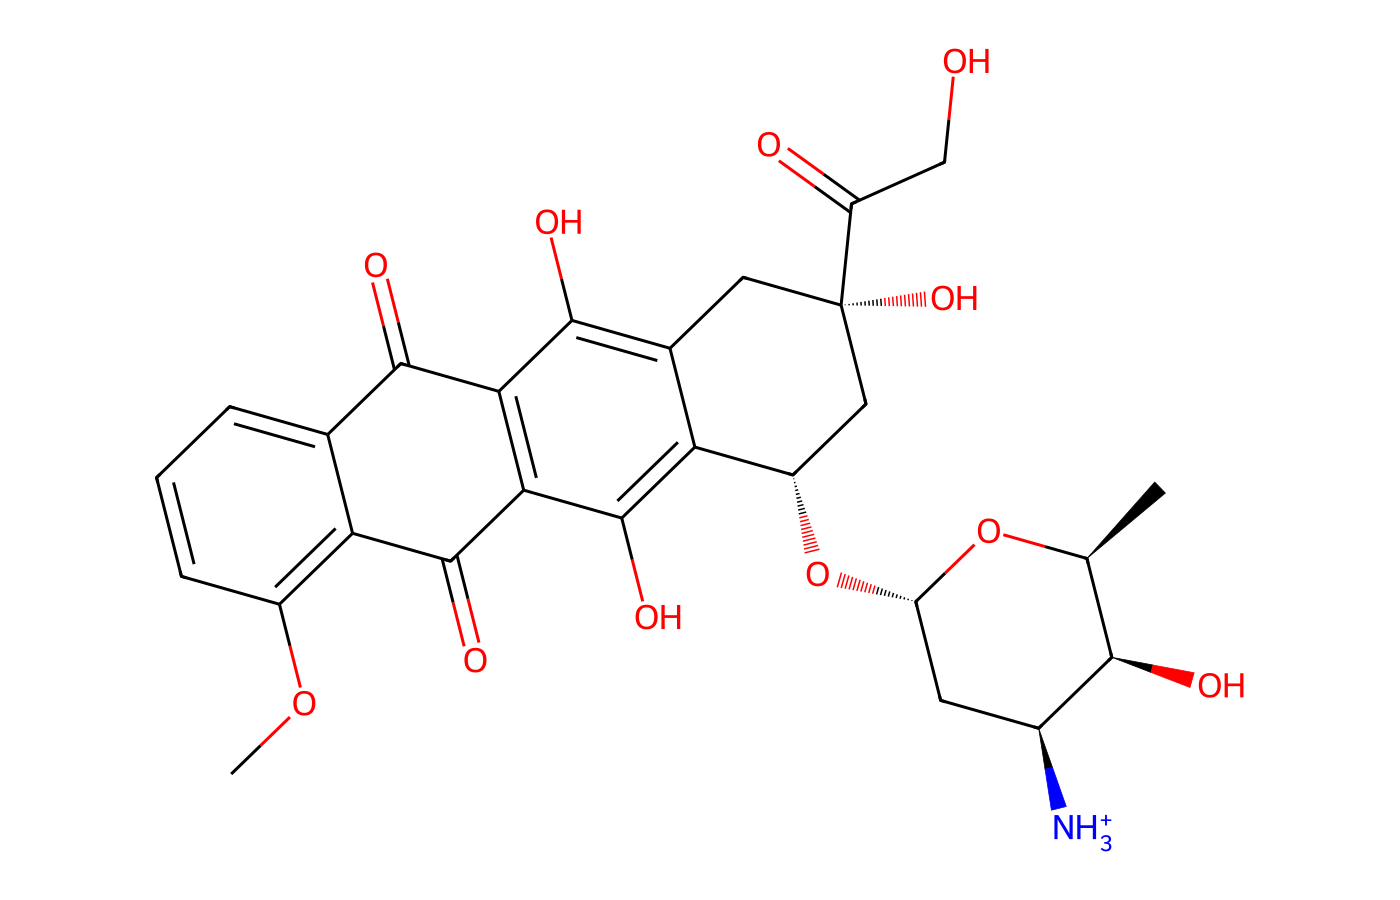
\includegraphics[width=0.62\linewidth]{fig_dox_structure.png}\par
\vspace{0.2cm}
{\small\itshape Protonated doxorubicin, C\textsubscript{27}H\textsubscript{30}NO\textsubscript{11}\textsuperscript{+}
 (net charge $+1$, \SI{544.5}{g\,mol^{-1}})\par}
\vfill
{\large Submitted by\par}
\vspace{0.2cm}
{\Large\bfseries \authorname\par}
\if\relax\detokenize\expandafter{\studentid}\relax\else{\large ID: \studentid\par}\fi
\vspace{0.5cm}
\if\relax\detokenize\expandafter{\coursename}\relax\else{\large \coursename\par}\fi
\if\relax\detokenize\expandafter{\supervisor}\relax\else{\large Under the supervision of \textbf{\supervisor}\par}\fi
\vspace{0.6cm}
{\large \institution\par}
{\normalsize \campus\par}
\vspace{0.4cm}
{\normalsize \reportdate\par}
\end{titlepage}

% ------------------------------ abstract ----------------------------
\pagenumbering{roman}
\section*{Abstract}
\addcontentsline{toc}{section}{Abstract}

Doxorubicin (DOX) is a frontline anthracycline anticancer drug whose clinical use is
limited by cardiotoxicity; encapsulating it in liposomes such as Doxil\textsuperscript{\textregistered}
improves its therapeutic index, and the lipid composition of the carrier is expected to govern how the
drug is retained and released. This project examines, at atomic resolution, how
cholesterol modifies the interaction of a single protonated doxorubicin molecule (\dox) with a
phosphatidylcholine membrane. Two systems were built with CHARMM-GUI and simulated with
GROMACS~2026 using the CHARMM36 lipid force field, CGenFF parameters for the drug and TIP3P water:
(\sysA) a pure DPPC bilayer in the fluid, liquid-disordered (\Ld) phase at \SI{323.15}{K}, and
(\sysB) an equimolar DPPC/cholesterol bilayer in the liquid-ordered (\Lo) phase at \SI{303.15}{K}.
Each system was simulated for \SI{150}{ns} of unrestrained NPT production, starting with \dox{} in the
aqueous phase, and analysed for drug position, binding kinetics, density profiles, orientation,
interaction energies, radial distribution functions, hydrogen bonding, lateral diffusion and lipid
chain order.

Both bilayers reproduce known structural properties: fluid DPPC gives an area per lipid of
\SI{61.0}{\angstrom^2}, a phosphate-to-phosphate thickness of \SI{39.6}{\angstrom} and a
plateau order parameter $-\scd \approx 0.22$, while 50\,\% cholesterol condenses the membrane to
\SI{39.2}{\angstrom^2} per molecule, thickens it to \SI{47.5}{\angstrom} and doubles the chain order
($-\scd \approx 0.43$). The drug behaves qualitatively differently in the two membranes. In fluid DPPC,
\dox{} anchors its ammonium group to the phosphates (N--O contact \SI{2.75}{\angstrom}, in agreement
with the \SI{2.65}{\angstrom} reported in the reference study), crosses the phosphate plane after
$\approx\SI{56}{ns}$ and then remains inserted for the rest of the run, with its centre
\SI{12}{\angstrom}--\SI{14}{\angstrom} from the bilayer midplane and its anthracycline ring tilted into the
upper acyl chains. The insertion is accompanied by a jump in the van der Waals interaction to
\SI{-44 \pm 7}{\kcal\per\mol} (reference: $\approx\SI{-39}{\kcal\per\mol}$) and a slow-down of lateral
diffusion by more than an order of magnitude. In the cholesterol-rich bilayer, \dox{} never penetrates:
it adsorbs and desorbs reversibly at the headgroup surface (12 binding events, mean residence
\SI{5.1}{ns}, bound 44\,\% of the time), spends 99\,\% of the trajectory outside the phosphate plane, and
its interaction with the membrane is less than half as strong. Cholesterol therefore acts as a barrier to
drug penetration by condensing and ordering the bilayer, consistent with experimental evidence and with
the free-energy trends reported by Siani \emph{et~al.} These results support the use of
cholesterol-rich formulations for drug retention in liposomal carriers, and point to lipid packing as the
key design variable.

\vspace{0.4em}
\noindent\textbf{Keywords:} doxorubicin; molecular dynamics; lipid bilayer; DPPC; cholesterol;
liquid-ordered phase; liposomal drug delivery; GROMACS; CHARMM36.

\clearpage
\begingroup\setstretch{1.0}\setlength{\parskip}{0pt}
\tableofcontents
\clearpage
\listoffigures
\listoftables
\endgroup

\section*{List of Abbreviations}
\addcontentsline{toc}{section}{List of Abbreviations}
{\small
\begin{tabular}{@{}p{1.9cm}p{5.6cm}@{\hspace{0.6cm}}p{1.9cm}p{5.6cm}@{}}
\dox & protonated doxorubicin & NPT & isothermal--isobaric ensemble \\
DPPC & 1,2-dipalmitoyl-\emph{sn}-glycero-3-phosphocholine & APL & area per lipid \\
CHL1 & cholesterol (CHARMM residue name) & $D_{\mathrm{PP}}$ & phosphate-to-phosphate thickness \\
\Ld{} / \Lo{} & liquid-disordered / liquid-ordered phase & RDF, $g(r)$ & radial distribution function \\
MD & molecular dynamics & MSD & mean-squared displacement \\
CGenFF & CHARMM General Force Field & $\scd$ & carbon--deuterium order parameter \\
PME & particle-mesh Ewald summation & COM & centre of mass \\
 & & LJ & Lennard-Jones (van der Waals) \\
\end{tabular}}

\clearpage
\pagenumbering{arabic}

% =====================================================================
\section{Introduction}
\label{sec:intro}

\subsection{Doxorubicin and the need for lipid carriers}
Doxorubicin (DOX) is an anthracycline antibiotic and one of the most widely prescribed chemotherapeutic
agents, used against breast carcinoma, osteosarcoma, acute leukaemias and several other cancers
\cite{minotti2004}. Its principal cytotoxic mechanism is intercalation of the planar
anthraquinone (aglycone) ring between DNA base pairs and the poisoning of topoisomerase~II, leading to
double-strand breaks and arrested replication. The action is, however, not selective: healthy tissues, the
heart in particular, are also damaged, and cumulative cardiotoxicity sets the maximum lifetime dose.

Encapsulation in liposomes is the most successful strategy to date for improving the therapeutic index of
DOX. The PEGylated liposomal formulation Doxil\textsuperscript{\textregistered}, the first nanodrug
approved by the U.S.\ FDA, prolongs circulation, accumulates passively in tumours through the enhanced
permeability and retention effect, and markedly reduces cardiac exposure \cite{barenholz2012}. Its
membrane is composed of a saturated phosphatidylcholine and roughly 40\,mol\,\% cholesterol.
That choice is not accidental: the composition and physical phase of the carrier membrane determine how
strongly the drug partitions into the bilayer, how fast it leaks, and how it is ultimately released.

\subsection{The molecular question}
At physiological pH the daunosamine sugar of DOX carries a protonated primary amine
($\mathrm{p}K_\mathrm{a}\approx 8.3$), so the molecule exists predominantly as the cation \dox{}. The
molecule is therefore amphiphilic: a charged, hydrogen-bonding sugar attached to a large, rigid and
partially hydrophobic tetracyclic ring system. Its interaction with a membrane is thus a balance between
(i) electrostatic attraction of the \nhthree{} group to the anionic phosphate groups of the lipid
headgroups and (ii) hydrophobic burial of the aglycone in the acyl-chain region. Both contributions are
expected to depend on lipid packing.

Cholesterol is the main regulator of packing in biological and liposomal membranes. Mixed with a saturated
phospholipid such as DPPC, it forms the liquid-ordered (\Lo) phase, in which chains are highly ordered
(as in a gel) but lipids still diffuse laterally (as in a fluid). The \Lo{} phase is thicker, more
condensed and less permeable than the liquid-disordered (\Ld) phase of pure fluid DPPC. Experiments have
shown that DOX penetrates more deeply into fluid than into gel-phase phosphatidylcholine membranes, and
that adding cholesterol reduces the overall DOX--membrane interaction \cite{siani2021,alves2017}.
Earlier simulations reported that the free-energy barrier to DOX translocation through DPPC increases with
cholesterol content \cite{yacoub2011}.

All-atom molecular dynamics (MD) simulations resolve these interactions at a level of detail that is
difficult to reach experimentally. The present project was designed as a reproduction and extension of the
DPPC part of the study by Siani \emph{et~al.} \cite{siani2021}, who simulated \dox{} with DPPC,
DPPC/cholesterol, sphingomyelin and sphingomyelin/cholesterol bilayers using NAMD.

\subsection{Objectives}
The aims of this project were:
\begin{enumerate}[label=\arabic*.]
  \item to build and equilibrate two all-atom membrane models that differ only in cholesterol content
        and phase: a fluid DPPC bilayer (\Ld, \SI{323.15}{K}; system \sysA) and an equimolar
        DPPC/cholesterol bilayer (\Lo, \SI{303.15}{K}; system \sysB), each containing one \dox{} molecule
        in the aqueous phase;
  \item to validate both membranes against experimental structural data (area per lipid, thickness,
        chain order parameters);
  \item to follow, without bias, how \dox{} approaches, binds to and penetrates each membrane, and to
        characterise its final location, orientation, interaction energetics, hydrogen bonding and
        mobility;
  \item to compare the outcome quantitatively with the reference study and to interpret the role of
        cholesterol for liposomal drug formulation;
  \item to go beyond the reference study with analyses it does not report, namely acyl-chain order
        parameters, binding kinetics, drug orientation and lateral diffusion (\cref{sec:beyond}).
\end{enumerate}

% =====================================================================
\section{Theoretical Background}
\label{sec:theory}

\subsection{Classical molecular dynamics}
MD integrates Newton's equations of motion, $m_i\,\ddot{\mathbf r}_i = -\nabla_i U(\{\mathbf r\})$, for
all atoms of a system, so that thermodynamic and dynamic properties can be obtained as time averages along
the trajectory. Here the leap-frog integrator was used with a time step of \SI{2}{fs}, made possible by
constraining bonds to hydrogen atoms with LINCS \cite{hess1997}.

\subsection{Force field}
The potential energy is given by an additive empirical force field of the CHARMM form:
\begin{equation}
\begin{aligned}
U ={}& \sum_{\text{bonds}} k_b (b-b_0)^2 + \sum_{\text{angles}} k_\theta(\theta-\theta_0)^2
      + \sum_{\text{dihedrals}} k_\phi\,[1+\cos(n\phi-\delta)]
      + \sum_{\text{impropers}} k_\omega(\omega-\omega_0)^2 \\
     &+ \sum_{i<j}\left\{ \varepsilon_{ij}\left[\left(\frac{R^{\min}_{ij}}{r_{ij}}\right)^{12}
      - 2\left(\frac{R^{\min}_{ij}}{r_{ij}}\right)^{6}\right]
      + \frac{q_i q_j}{4\pi\varepsilon_0 r_{ij}} \right\}.
\end{aligned}
\label{eq:ff}
\end{equation}
CHARMM36 \cite{klauda2010} was used for DPPC and cholesterol, CGenFF \cite{vanommeslaeghe2010} for
\dox{} (parameters assigned by analogy through the CHARMM-GUI Ligand Reader \cite{kim2017}), and the
CHARMM-modified TIP3P model \cite{jorgensen1983} for water. Lennard-Jones forces were smoothly switched
to zero between \SI{1.0}{nm} and \SI{1.2}{nm} (force switch \cite{steinbach1994}), the cut-off scheme
with which CHARMM36 lipids were parameterised. Long-range electrostatics were computed with smooth
particle-mesh Ewald (PME) summation \cite{essmann1995} with a real-space cut-off of \SI{1.2}{nm}.

\subsection{Temperature and pressure control}
Temperature was maintained with the stochastic velocity-rescaling thermostat \cite{bussi2007}, which
samples the canonical distribution correctly. Pressure was controlled at \SI{1}{bar} with the stochastic
cell-rescaling (C-rescale) barostat \cite{bernetti2020} in semi-isotropic mode, in which the membrane
plane ($xy$) and the normal ($z$) are scaled independently, so that the bilayer area can relax freely
(tensionless membrane).

\subsection{Analysis observables}
\paragraph{Area per lipid and thickness.}
For a bilayer with $N_\mathrm{leaf}$ molecules per leaflet in a box of lateral dimensions $L_x\times L_y$,
\begin{equation}
  \mathrm{APL} = \frac{L_x L_y}{N_\mathrm{leaf}} .
\end{equation}
The phosphate-to-phosphate thickness $D_\mathrm{PP}$ is the distance between the mean $z$-positions of
the phosphorus atoms in the two leaflets.

\paragraph{Order parameter.}
The orientational order of the acyl chains is quantified by
\begin{equation}
  \scd = \left\langle \frac{3\cos^2\beta - 1}{2} \right\rangle ,
  \label{eq:scd}
\end{equation}
where $\beta$ is the angle between a C--H bond vector and the bilayer normal and the average runs over
lipids, equivalent hydrogens and time \cite{vermeer2007}. The quantity $-\scd$ can be compared directly
with deuterium NMR measurements \cite{seelig1974}; it ranges from 0 (isotropic) to 0.5 (fully ordered
all-\emph{trans} chain).

\paragraph{Density profiles.}
Number densities of selected atom groups were histogrammed along $z$ relative to the instantaneous bilayer
centre, $\rho_k(z) = \langle N_k(z, z+\Delta z)\rangle / (L_xL_y\Delta z)$, and symmetrised about the
midplane.

\paragraph{Radial distribution function.}
For a reference atom (the \dox{} ammonium nitrogen) and a set of target atoms $B$,
\begin{equation}
  g(r) = \frac{\langle n_B(r, r+\Delta r)\rangle}{4\pi r^2 \Delta r\,\rho_B},
\end{equation}
where $\rho_B$ is the mean number density of $B$ in the box.

\paragraph{Hydrogen bonds.}
A hydrogen bond D--H$\cdots$A was counted when the donor--acceptor distance was below
\SI{3.5}{\angstrom} and the D--H$\cdots$A angle exceeded \SI{150}{\degree}.

\paragraph{Lateral diffusion.}
The in-plane self-diffusion coefficient follows from the Einstein relation in two dimensions,
\begin{equation}
  \langle |\mathbf{r}_{xy}(t+\tau) - \mathbf{r}_{xy}(t)|^2 \rangle = 4D\tau ,
  \label{eq:msd}
\end{equation}
applied to the \dox{} centre of mass after removing the drift of the membrane.

\paragraph{Interaction energies.}
The \dox{}--lipid interaction was decomposed into short-range Coulomb and Lennard-Jones contributions
by recomputing energies over the stored trajectory with energy groups (\texttt{gmx mdrun -rerun}).

% =====================================================================
\section{Methodology}
\label{sec:methods}

In outline, the study had four stages. First, the drug was converted to its protonated form and given
CGenFF parameters. Second, two bilayers, pure DPPC (\sysA) and DPPC/cholesterol 1:1 (\sysB), were built
with CHARMM-GUI, and one \dox{} molecule was placed in the water above each. Third, both systems were
minimised, equilibrated with restraints that were released step by step, and then simulated without any
bias for \SI{150}{ns}. Finally, the trajectories were analysed for drug position, energetics, contacts and
mobility, and for membrane structure. \Cref{fig:workflow} summarises this workflow, and the following
subsections describe each stage.

\subsection{Preparation of protonated doxorubicin}
The three-dimensional conformer of doxorubicin was obtained from PubChem (CID~31703) \cite{pubchem2023}.
Because the daunosamine amine is protonated at physiological pH, the neutral structure was converted to
\dox{} with a short RDKit \cite{rdkit} script (\texttt{protonate.py}). The script removes hydrogens,
identifies the single primary aliphatic amine with the SMARTS pattern
\texttt{[NX3;H2;!\$(N-C=O)]}, sets its formal charge to $+1$, and re-adds all hydrogens with
three-dimensional coordinates. This gives C\textsubscript{27}H\textsubscript{30}NO\textsubscript{11}\textsuperscript{+}
(69 atoms, net charge $+1$; \cref{fig:dox}).

\begin{figure}[!htbp]
\centering
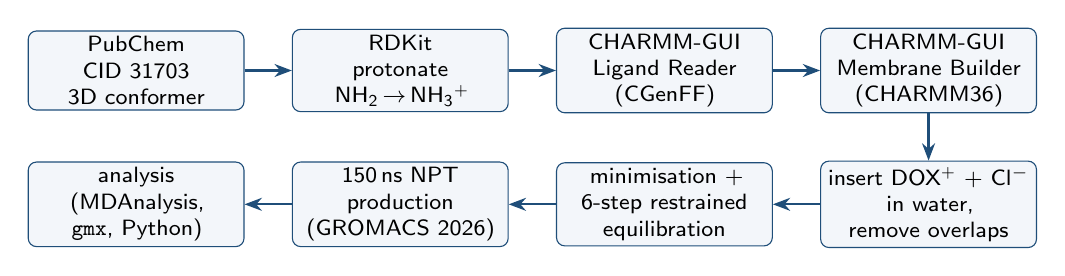
\begin{tikzpicture}[
  node distance=4mm and 6mm,
  box/.style={draw=accent, rounded corners=3pt, fill=boxbg, align=center,
              font=\sffamily\footnotesize, minimum height=10mm, text width=26mm, inner sep=2pt},
  arr/.style={-{Stealth[length=2.2mm]}, thick, accent}]
\node[box] (lig) {PubChem CID 31703\\3D conformer};
\node[box, right=of lig] (prot) {RDKit\\protonate NH\textsubscript{2}\,$\to$\,\nhthree};
\node[box, right=of prot] (cgenff) {CHARMM-GUI\\Ligand Reader\\(CGenFF)};
\node[box, right=of cgenff] (mem) {CHARMM-GUI\\Membrane Builder\\(CHARMM36)};
\node[box, below=6mm of mem] (ins) {insert \dox{} + Cl\textsuperscript{$-$}\\in water,\\remove overlaps};
\node[box, left=of ins] (eq) {minimisation +\\6-step restrained\\equilibration};
\node[box, left=of eq] (prod) {\SI{150}{ns} NPT\\production\\(GROMACS 2026)};
\node[box, left=of prod] (ana) {analysis\\(MDAnalysis,\\\texttt{gmx}, Python)};
\draw[arr] (lig) -- (prot); \draw[arr] (prot) -- (cgenff); \draw[arr] (cgenff) -- (mem);
\draw[arr] (mem) -- (ins); \draw[arr] (ins) -- (eq); \draw[arr] (eq) -- (prod); \draw[arr] (prod) -- (ana);
\end{tikzpicture}
\caption[Simulation workflow]{Workflow followed for both systems.}
\label{fig:workflow}
\end{figure}


Force-field parameters were generated with the CHARMM-GUI Ligand Reader \& Modeler \cite{kim2017},
which assigns CGenFF atom types, charges and parameters by analogy. The reported penalties were
28.5 (parameters) and 8.7 (charges). Penalties below 50 are conventionally considered acceptable for
use with only basic validation, and the highest-penalty term was a dihedral of the conjugated quinone
ring.

\begin{figure}[!htbp]
\centering
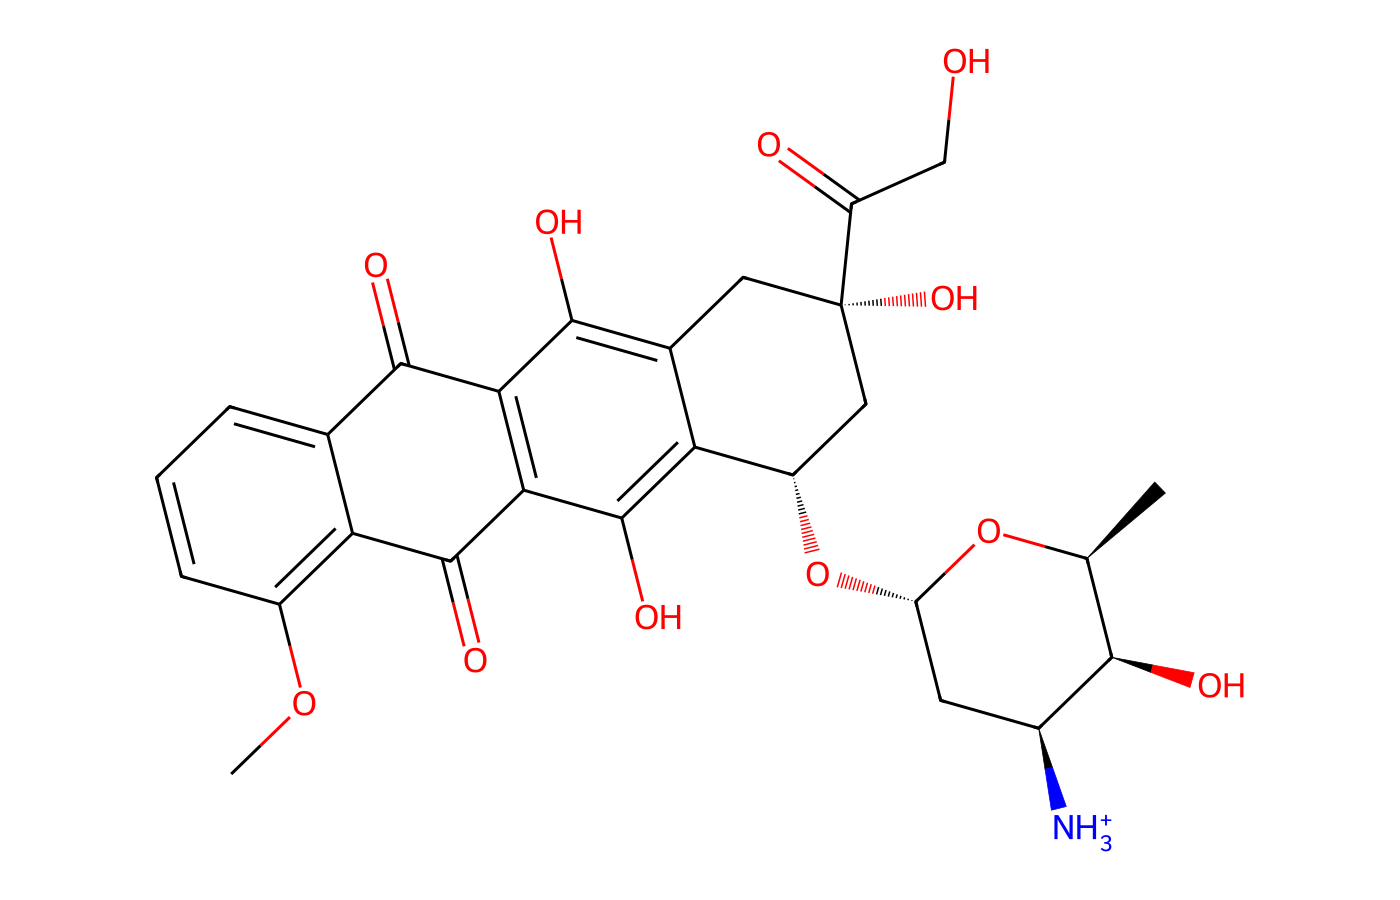
\includegraphics[width=0.66\linewidth]{fig_dox_structure.png}
\caption[Chemical structure of protonated doxorubicin]{Protonated doxorubicin (\dox) as simulated. The
planar tetracyclic anthraquinone (aglycone) is joined through a glycosidic bond to the daunosamine sugar,
which carries the \nhthree{} group that anchors the drug to the lipid phosphates. Drawn with RDKit from
\texttt{DOX\_plus.sdf}.}
\label{fig:dox}
\end{figure}

\subsection{Membrane systems}
Both bilayers were assembled with the CHARMM-GUI Membrane Builder \cite{jo2008,wu2014,lee2016}. A
single \dox{} molecule and one Cl\textsuperscript{$-$} counter-ion were then added to the water
layer, and overlapping water molecules were removed. The two systems are summarised in
\cref{tab:systems}. Their temperatures were chosen to match the reference study: \SI{323.15}{K} lies
well above the DPPC main transition (\SI{314}{K}), giving a fluid \Ld{} bilayer, while at
\SI{303.15}{K} the 1:1 DPPC/cholesterol mixture is in the \Lo{} phase.

For system \sysB{}, the cholesterol-containing bilayer was first equilibrated on its own, through the
full six-step protocol followed by an additional \SI{10}{ns} of unrestrained NPT, before the drug
was inserted. This ensured that cholesterol had relaxed within the leaflets.

\begin{table}[!htbp]
\centering
\caption[Composition of the simulated systems]{Composition and dimensions of the two simulated systems.
Box dimensions are averages over the production run.}
\label{tab:systems}
\begin{tabular}{@{}lcc@{}}
\toprule
 & \textbf{System \sysA} & \textbf{System \sysB} \\
\midrule
Membrane            & pure DPPC            & DPPC/cholesterol 1:1 \\
Lipid phase         & liquid-disordered (\Ld) & liquid-ordered (\Lo) \\
Temperature         & \SI{323.15}{K}       & \SI{303.15}{K} \\
DPPC                & 128 (64 per leaflet) & 64 (32 per leaflet) \\
Cholesterol         & 0                    & 64 (32 per leaflet) \\
TIP3P water         & 5354                 & 4454 \\
Water / lipid ratio & 41.8                 & 34.8 \\
\dox{} / Cl\textsuperscript{$-$} & 1 / 1   & 1 / 1 \\
Total atoms         & \num{32772}          & \num{26488} \\
Box $L_x = L_y$ (nm) & 6.25                & 5.01 \\
Box $L_z$ (nm)      & 8.12                 & 9.85 \\
Initial \dox{} height above midplane & \SI{29.6}{\angstrom} & \SI{40.3}{\angstrom} \\
Production length   & \SI{150}{ns}         & \SI{150}{ns} \\
\bottomrule
\end{tabular}
\end{table}

\subsection{Energy minimisation and equilibration}
Each system was energy-minimised by steepest descent (5000 steps) and then equilibrated with the standard
CHARMM-GUI six-step protocol. In this protocol, positional restraints on the lipid headgroups and
dihedral restraints on the lipid glycerol/double-bond geometry are released gradually
(\cref{tab:equil}). The first two steps are run at constant volume, and the remaining steps at constant
pressure.

\begin{table}[!htbp]
\centering
\caption[Equilibration protocol]{Minimisation and equilibration protocol. Force constants are in
\si{kJ\,mol^{-1}\,nm^{-2}} (positional) and \si{kJ\,mol^{-1}\,rad^{-2}} (dihedral).}
\label{tab:equil}
\begin{tabular}{@{}lcccccc@{}}
\toprule
Step & Ensemble & $\Delta t$ (fs) & Steps & Time (ns) & Lipid pos.\ restr. & Dihedral restr. \\
\midrule
6.0 minimisation & --  & --  & 5000   & --     & 1000 & 1000 \\
6.1              & NVT & 1   & 125000 & 0.125  & 1000 & 1000 \\
6.2              & NVT & 1   & 125000 & 0.125  & 400  & 400  \\
6.3              & NPT & 1   & 125000 & 0.125  & 400  & 200  \\
6.4              & NPT & 2   & 250000 & 0.5    & 200  & 200  \\
6.5              & NPT & 2   & 250000 & 0.5    & 40   & 100  \\
6.6              & NPT & 2   & 250000 & 0.5    & 0    & 0    \\
\midrule
\multicolumn{4}{@{}l}{Total restrained/relaxation equilibration} & 1.875 & & \\
\bottomrule
\end{tabular}
\end{table}

\subsection{Production simulations}
Production runs were carried out with GROMACS~2026.4 \cite{abraham2015} using the parameters in
\cref{tab:mdp}. The two systems differ only in reference temperature. Coordinates were written every
\SI{10}{ps}, giving \num{15001} frames per system. The runs were performed in several restart segments
from checkpoint files, and the segments were concatenated for analysis.

\begin{table}[!htbp]
\centering
\caption[Production MD parameters]{Production MD parameters (identical for both systems except $T$).}
\label{tab:mdp}
\begin{tabularx}{0.92\linewidth}{@{}lX@{}}
\toprule
Parameter & Setting \\
\midrule
Integrator, time step & leap-frog (\texttt{md}), \SI{2}{fs} \\
Constraints & LINCS on bonds to H atoms \\
Neighbour searching & Verlet buffer, \texttt{nstlist}\,=\,20, $r_\mathrm{list}=\SI{1.2}{nm}$ \\
Van der Waals & cut-off \SI{1.2}{nm}, force-switch from \SI{1.0}{nm} \\
Electrostatics & PME, real-space cut-off \SI{1.2}{nm} \\
Thermostat & velocity rescaling, $\tau_T=\SI{1.0}{ps}$; groups membrane (+\dox) and solvent \\
Temperature & \SI{323.15}{K} (\sysA), \SI{303.15}{K} (\sysB) \\
Barostat & C-rescale, semi-isotropic, $\tau_P=\SI{5.0}{ps}$, $P=\SI{1.0}{bar}$,
           compressibility \SI{4.5e-5}{bar^{-1}} \\
COM motion removal & linear, separately for membrane and solvent, every 100 steps \\
Output & compressed coordinates every \SI{10}{ps}; energies every \SI{2}{ps} \\
Length & $5\times10^7$ steps = \SI{100}{ns}, extended to \SI{150}{ns} \\
\bottomrule
\end{tabularx}
\end{table}

\subsection{Trajectory analysis}
All analyses used custom Python scripts built on MDAnalysis \cite{michaudagrawal2011,gowers2016}, NumPy
and Matplotlib \cite{hunter2007}, together with GROMACS tools. The bilayer centre was defined in each
frame as the periodic (circular) mean of the $z$-coordinates of all lipid atoms, which is robust when the
membrane drifts across the periodic boundary. The analyses performed were:
\begin{itemize}
  \item \textbf{Drug tracking} (\texttt{track.py}, \texttt{track\_B.py}): the height of the \dox{}
        centre above the bilayer midplane, $D_\mathrm{PP}$, the minimum \dox{}--phosphorus distance and,
        for \sysB{}, the minimum \dox{}--cholesterol-oxygen distance, for every frame.
  \item \textbf{Binding kinetics} (\texttt{kinetics.py}): \dox{} was classified as \emph{bound} when
        any of its atoms was within \SI{5}{\angstrom} of a lipid phosphorus. Excursions shorter than
        \SI{1}{ns} were merged into the surrounding state. Residence times and an apparent
        bound/unbound ratio were then extracted.
  \item \textbf{Region occupancy and crossing} (\texttt{cross.py}): the fraction of time spent in water,
        in the headgroup region, in the upper tails and in the core, and detection of any leaflet-to-leaflet
        crossing.
  \item \textbf{Density profiles} (\texttt{density.py}) for water oxygen, phosphorus, acyl-tail carbons,
        cholesterol O3 and \dox{}, over the final bound period of each system.
  \item \textbf{Orientation} (\texttt{orient.py}): the heights of the \nhthree{} nitrogen and of the
        heavy atom farthest from it (on the anthracycline ring), and the angle of the N$\to$ring vector
        with respect to the inward bilayer normal.
  \item \textbf{RDFs} (\texttt{rdf.py}) between the \nhthree{} nitrogen and phosphate oxygens, ester
        (carbonyl/glycerol) oxygens, water oxygens and the cholesterol hydroxyl.
  \item \textbf{Hydrogen bonds} (\texttt{hbonds.py}) donated by \dox{} (\nhthree{} and hydroxyl groups) to
        phosphate O, ester O, cholesterol O and water.
  \item \textbf{Interaction energies}: \texttt{gmx mdrun -rerun} with energy groups for \dox{} and the membrane
        (\sysA), and for \dox{}, DPPC and cholesterol separately (\sysB).
  \item \textbf{Lateral diffusion} (\texttt{msd.py}): Eq.~\eqref{eq:msd} fitted between \SI{0.1}{ns} and
        one fifth of each window, on windows where \dox{} stayed in a single state.
  \item \textbf{Membrane structure}: APL from the box dimensions, and $\scd$ (Eq.~\eqref{eq:scd}) for
        carbons 2--16 of both chains (\texttt{scd.py}).
\end{itemize}

\subsection{Computational resources}
All simulations were run locally on an Apple~M4 workstation (10 CPU cores) with the Homebrew build of
GROMACS~2026.4. Throughput was \SIrange{20.5}{21.8}{ns/day} for system \sysA{} (\num{32772} atoms) and
\SIrange{24.1}{26.2}{ns/day} for system \sysB{} (\num{26488} atoms). The two \SI{150}{ns} production
runs therefore needed about 13 days of wall-clock time in total. Trajectory snapshots and movies were
rendered with UCSF ChimeraX \cite{pettersen2021}.

% =====================================================================
\section{Results}
\label{sec:results}

\subsection{Validation of the membrane models}
Before interpreting drug behaviour, the two membranes were checked against known properties
(\cref{tab:membrane}). Temperature control was tight in both runs, at \SI{323.2 \pm 2.0}{K} and
\SI{303.2 \pm 2.1}{K}.

\begin{table}[!htbp]
\centering
\caption[Structural properties of the bilayers]{Structural properties of the two membranes over the
production runs (mean $\pm$ standard deviation). Experimental values for fluid DPPC at
\SI{323}{K} are from Ku\v{c}erka \emph{et~al.} \cite{kucerka2011} and Seelig \& Seelig \cite{seelig1974}.}
\label{tab:membrane}
\begin{tabular}{@{}lccc@{}}
\toprule
Property & \sysA: DPPC (\Ld) & \sysB: DPPC/chol (\Lo) & Exp.\ DPPC, \SI{323}{K} \\
\midrule
Area per molecule (\si{\angstrom^2}) & \num{61.0 \pm 1.3} & \num{39.2 \pm 0.3} & \num{63.0 \pm 1.0} \\
Area per DPPC, box/32 (\si{\angstrom^2}) & -- & \num{78.4} & -- \\
$D_\mathrm{PP}$ (\si{\angstrom}) & \num{39.6} & \num{47.5} & $\approx 38$ \\
$-\scd$ plateau, C4--C10, \emph{sn}-2 & \num{0.225} & \num{0.432} & $\approx 0.20$--$0.22$ \\
$-\scd$ plateau, C4--C10, \emph{sn}-1 & \num{0.214} & \num{0.430} & -- \\
Maximum $-\scd$ & \num{0.236} & \num{0.448} & -- \\
\bottomrule
\end{tabular}
\end{table}

Fluid DPPC reproduces the experimental area per lipid to within 3\,\%, and its thickness and plateau order
parameter are also consistent with experiment, as expected for CHARMM36 \cite{klauda2010}. Adding 50\,\%
cholesterol has three effects:
\begin{itemize}
  \item the area per molecule shrinks by 36\,\% (the well-known \emph{condensing effect});
  \item the bilayer becomes \SI{8}{\angstrom} thicker;
  \item the chain order roughly doubles (\cref{fig:scd}).
\end{itemize}
The order-parameter profile of \sysB{} is high ($-\scd \approx 0.43$--$0.45$) along carbons 4--11, where
the rigid cholesterol ring system lies alongside the DPPC chains, and it falls off only towards the chain
ends. This is the signature of the liquid-ordered phase. The two membranes therefore provide the intended
contrast: a loosely packed fluid bilayer and a tightly packed, ordered one.

\begin{figure}[!htbp]
\centering
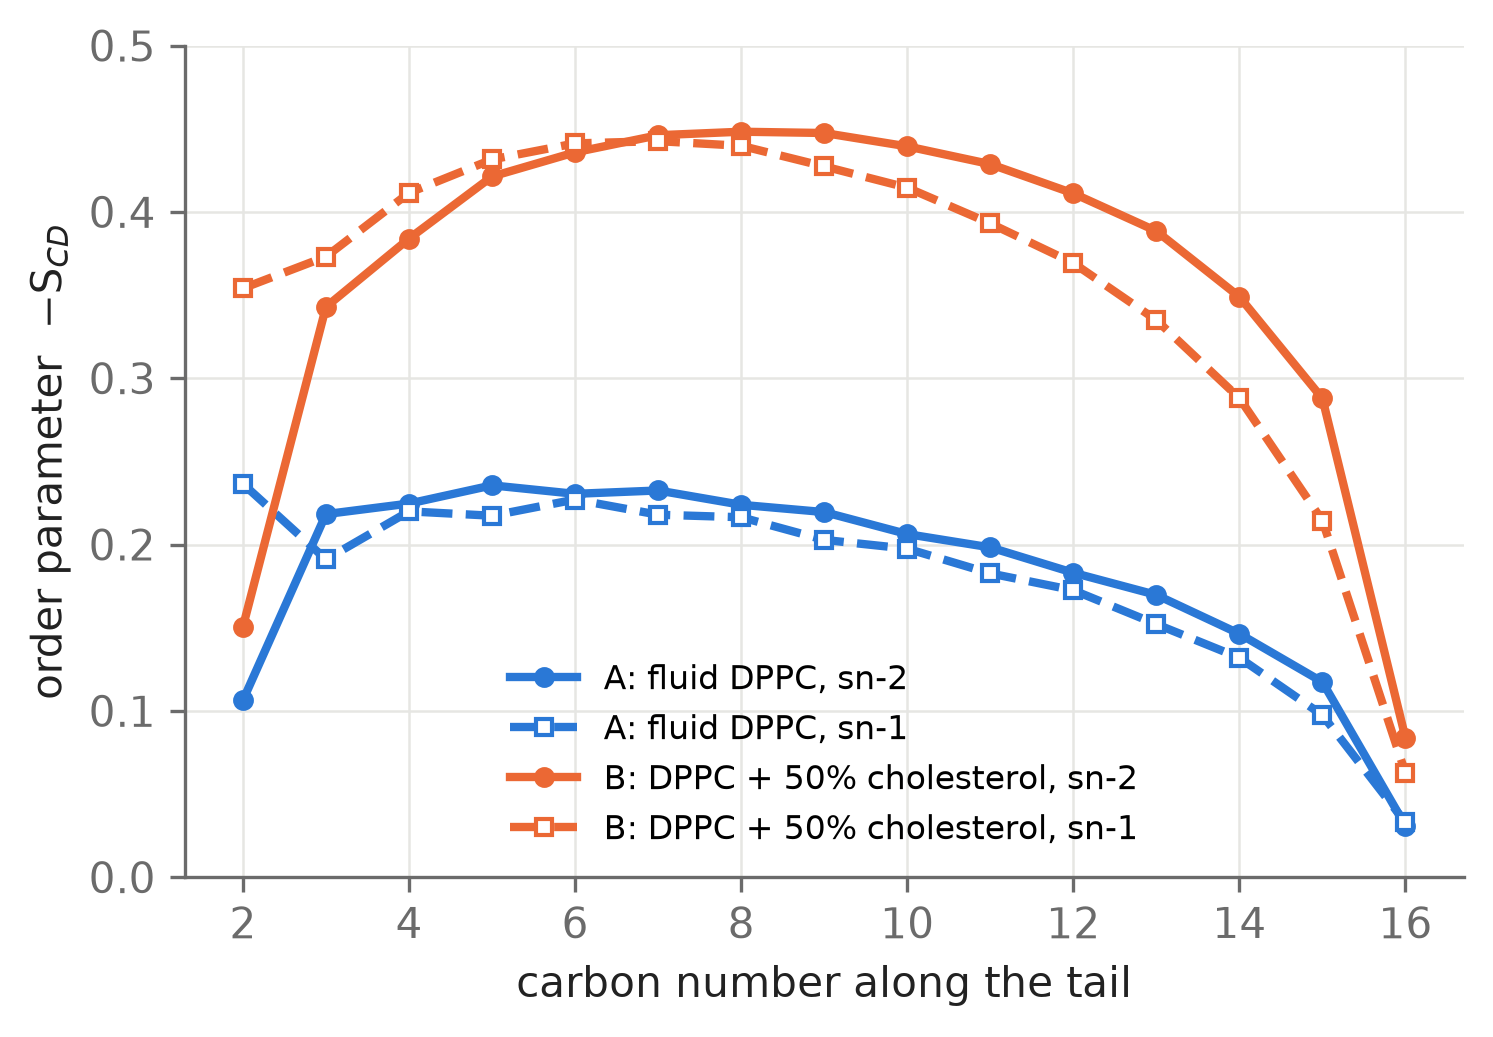
\includegraphics[width=0.66\linewidth]{fig5_order_parameter.png}
\caption[Acyl-chain order parameters]{Deuterium order parameter $-\scd$ along the \emph{sn}-1 and
\emph{sn}-2 chains of DPPC. Cholesterol (orange) roughly doubles the order of the chain segments
adjacent to its rigid ring system (C4--C11), which is characteristic of the liquid-ordered phase.}
\label{fig:scd}
\end{figure}

\subsection{Approach, binding and penetration of \texorpdfstring{\dox}{DOX+}}
\Cref{fig:depth} shows the height of the \dox{} centre above the bilayer midplane over the whole
\SI{150}{ns} for both systems, and \cref{fig:timeline} shows when the drug was in contact with the
membrane. Representative snapshots appear in \cref{fig:snapA,fig:snapB}, and the binding statistics are
collected in \cref{tab:kinetics}.

\begin{figure}[!htbp]
\centering
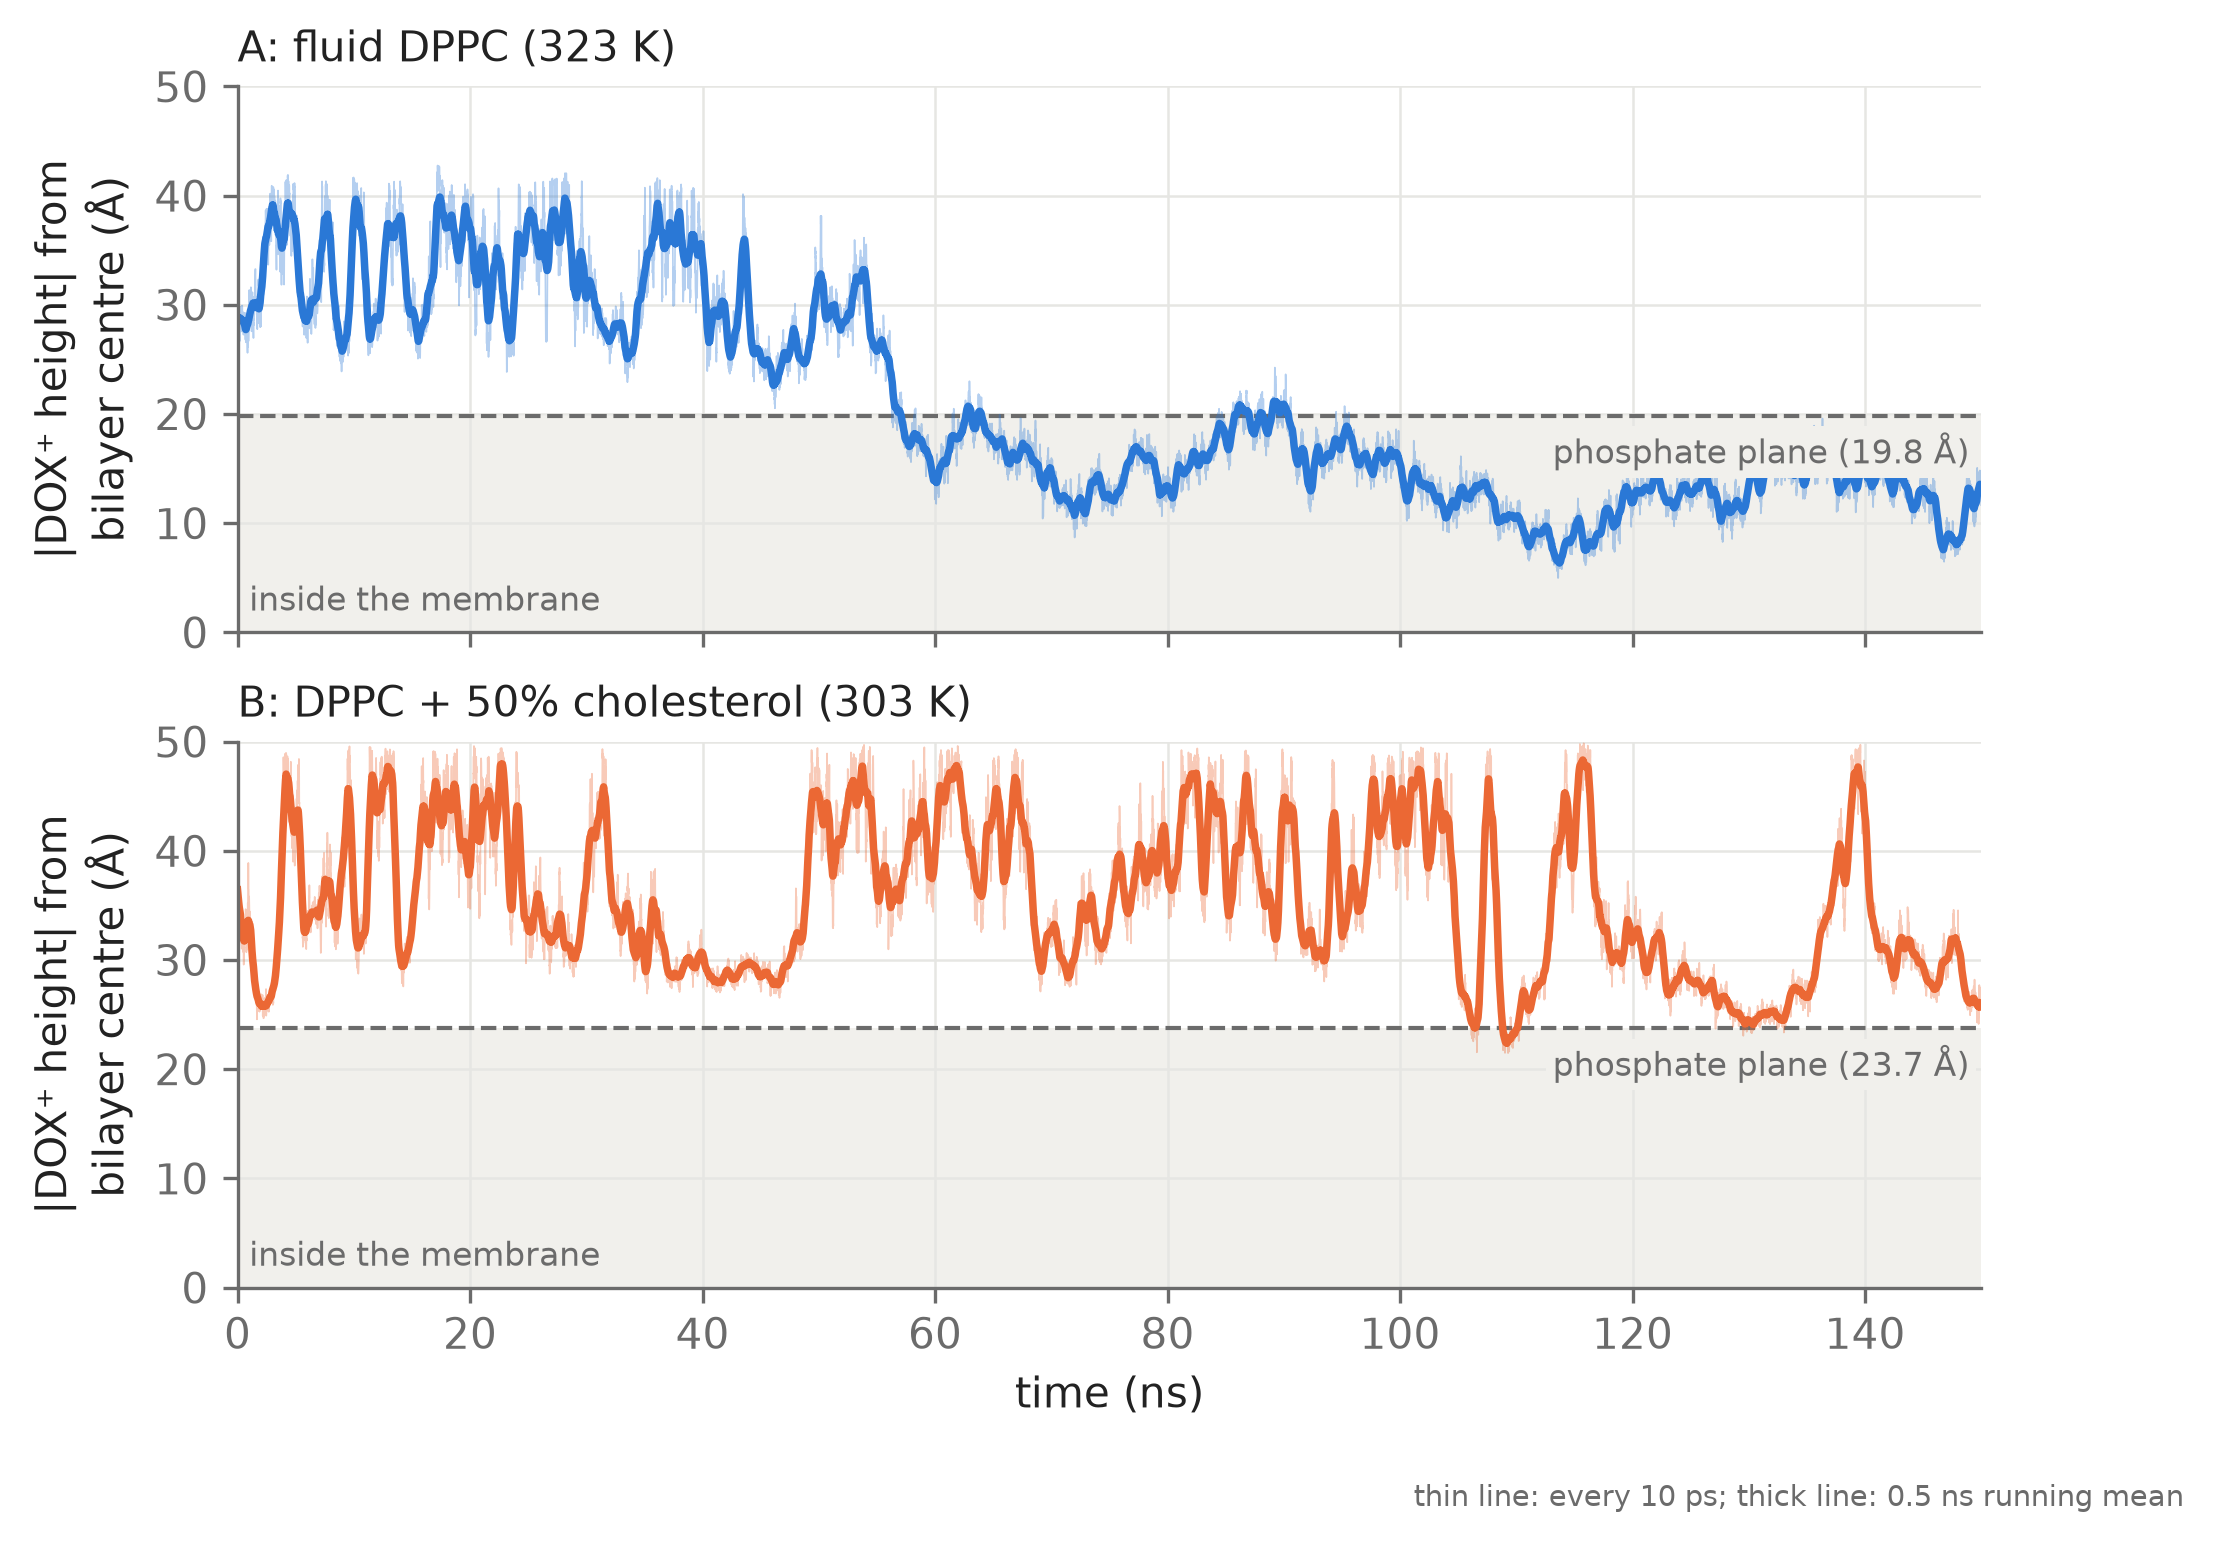
\includegraphics[width=0.92\linewidth]{fig1_depth_vs_time.png}
\caption[\dox{} height above the bilayer centre versus time]{Distance of the \dox{} centre from the bilayer
midplane. The dashed line marks the mean phosphate plane ($D_\mathrm{PP}/2$), and the shaded area is the
membrane interior. In fluid DPPC (\sysA) the drug crosses the phosphate plane at
$\approx\SI{56}{ns}$ and remains inserted. In DPPC/cholesterol (\sysB) it repeatedly visits the surface
but never passes the phosphates.}
\label{fig:depth}
\end{figure}

\begin{figure}[!htbp]
\centering
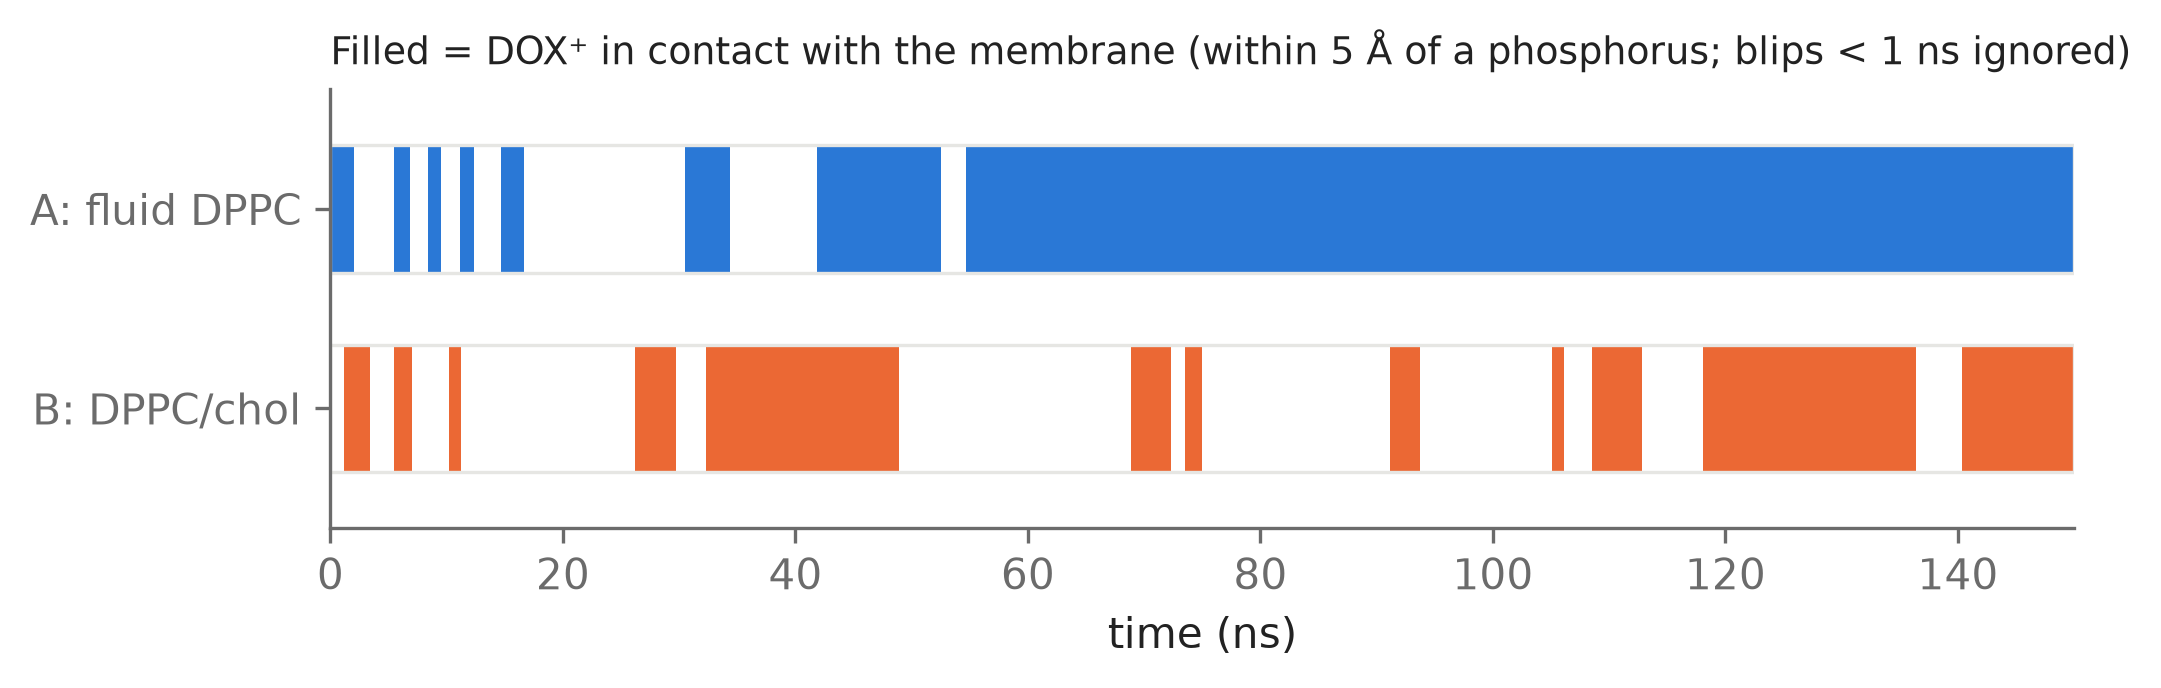
\includegraphics[width=0.95\linewidth]{fig2_binding_timeline.png}
\caption[Membrane-binding timeline]{Periods during which \dox{} is in contact with the membrane (any atom
within \SI{5}{\angstrom} of a phosphorus; blips shorter than \SI{1}{ns} ignored). In \sysA{}, binding
becomes permanent after $\approx\SI{55}{ns}$. In \sysB{}, binding is intermittent and reversible
throughout.}
\label{fig:timeline}
\end{figure}

\paragraph{System A: fluid DPPC.}
The trajectory shows three stages.
\begin{enumerate}[label=(\roman*)]
  \item \textbf{Surface sampling, 0--\SI{55}{ns}.} \dox{} explores the water layer and makes brief contacts
        with the headgroups (eight binding events, mean residence \SI{3.4}{ns}). Its mean height in the
        first \SI{50}{ns} is \SI{32.1 \pm 5.0}{\angstrom}.
  \item \textbf{Insertion, $\approx$\SIrange{55}{60}{ns}.} The drug stays anchored at the interface and
        crosses the phosphate plane (\SI{19.8}{\angstrom}) for the first time at \SI{56.3}{ns}.
  \item \textbf{Inserted state, 60--\SI{150}{ns}.} \dox{} never returns to the water. It is in contact
        with the membrane in 100\,\% of frames, and its centre sits at
        \SI{14.0 \pm 3.2}{\angstrom} from the midplane, settling to \SI{12.3 \pm 2.5}{\angstrom} over the
        last \SI{50}{ns}.
\end{enumerate}
The deepest excursion reached \SI{5.0}{\angstrom} from the midplane at \SI{113.6}{ns}. The drug never
entered the central \SI{5}{\angstrom} of the bilayer and never crossed to the opposite leaflet. Over the
whole run it spent 52\,\% of the time in the headgroup/glycerol region and 7\,\% in the upper acyl chains.

\paragraph{System B: DPPC/cholesterol.}
\dox{} binds and unbinds repeatedly throughout. There were 12 binding events, the longest lasting
\SIrange{16}{18}{ns}, with a mean residence time of \SI{5.1}{ns} and a mean time to rebind from water of
\SI{7.5}{ns}. The drug was in contact with the membrane for 44\,\% of the run and attached to both
leaflets (through the periodic water layer), as shown in \cref{fig:snapB}(d). It was below the phosphate
plane (\SI{23.7}{\angstrom}) in only 1.1\,\% of frames, and its deepest point was
\SI{21.5}{\angstrom}, just inside the phosphates. Even in the longest bound period
(\SIrange{118}{136}{ns}) its centre stayed \emph{outside} the phosphate plane, at
\SI{27.7 \pm 2.7}{\angstrom}.

\begin{table}[!htbp]
\centering
\caption[Binding and penetration statistics]{Binding and penetration statistics over \SI{150}{ns}.
``Bound'': any \dox{} atom within \SI{5}{\angstrom} of a lipid phosphorus (events $<\SI{1}{ns}$ merged).
The apparent $\Delta G = -k_\mathrm{B}T\ln(p_\mathrm{bound}/p_\mathrm{free})$ depends on box size and is
an order-of-magnitude indicator only.}
\label{tab:kinetics}
\begin{tabular}{@{}lcc@{}}
\toprule
Quantity & \sysA: DPPC & \sysB: DPPC/chol \\
\midrule
Fraction of time bound & 78\,\% & 44\,\% \\
Binding events & 8 & 12 \\
Mean residence time of transient binding & \SI{3.4}{ns} & \SI{5.1}{ns} \\
Mean time to rebind from water & \SI{4.6}{ns} & \SI{7.5}{ns} \\
Permanent binding from & $\approx$\,\SI{55}{ns} & never \\
First crossing of the phosphate plane & \SI{56.3}{ns} & \SI{106.1}{ns} (transient) \\
Time below the phosphate plane & 59\,\% & 1.1\,\% \\
Deepest point from midplane & \SI{5.0}{\angstrom} & \SI{21.5}{\angstrom} \\
Leaflet crossing (flip-flop) & no & no \\
Apparent $\Delta G_\mathrm{bind}$ & \SI{-0.8}{\kcal\per\mol} & \SI{+0.1}{\kcal\per\mol} \\
\bottomrule
\end{tabular}
\end{table}

\begin{figure}[!htbp]
\centering
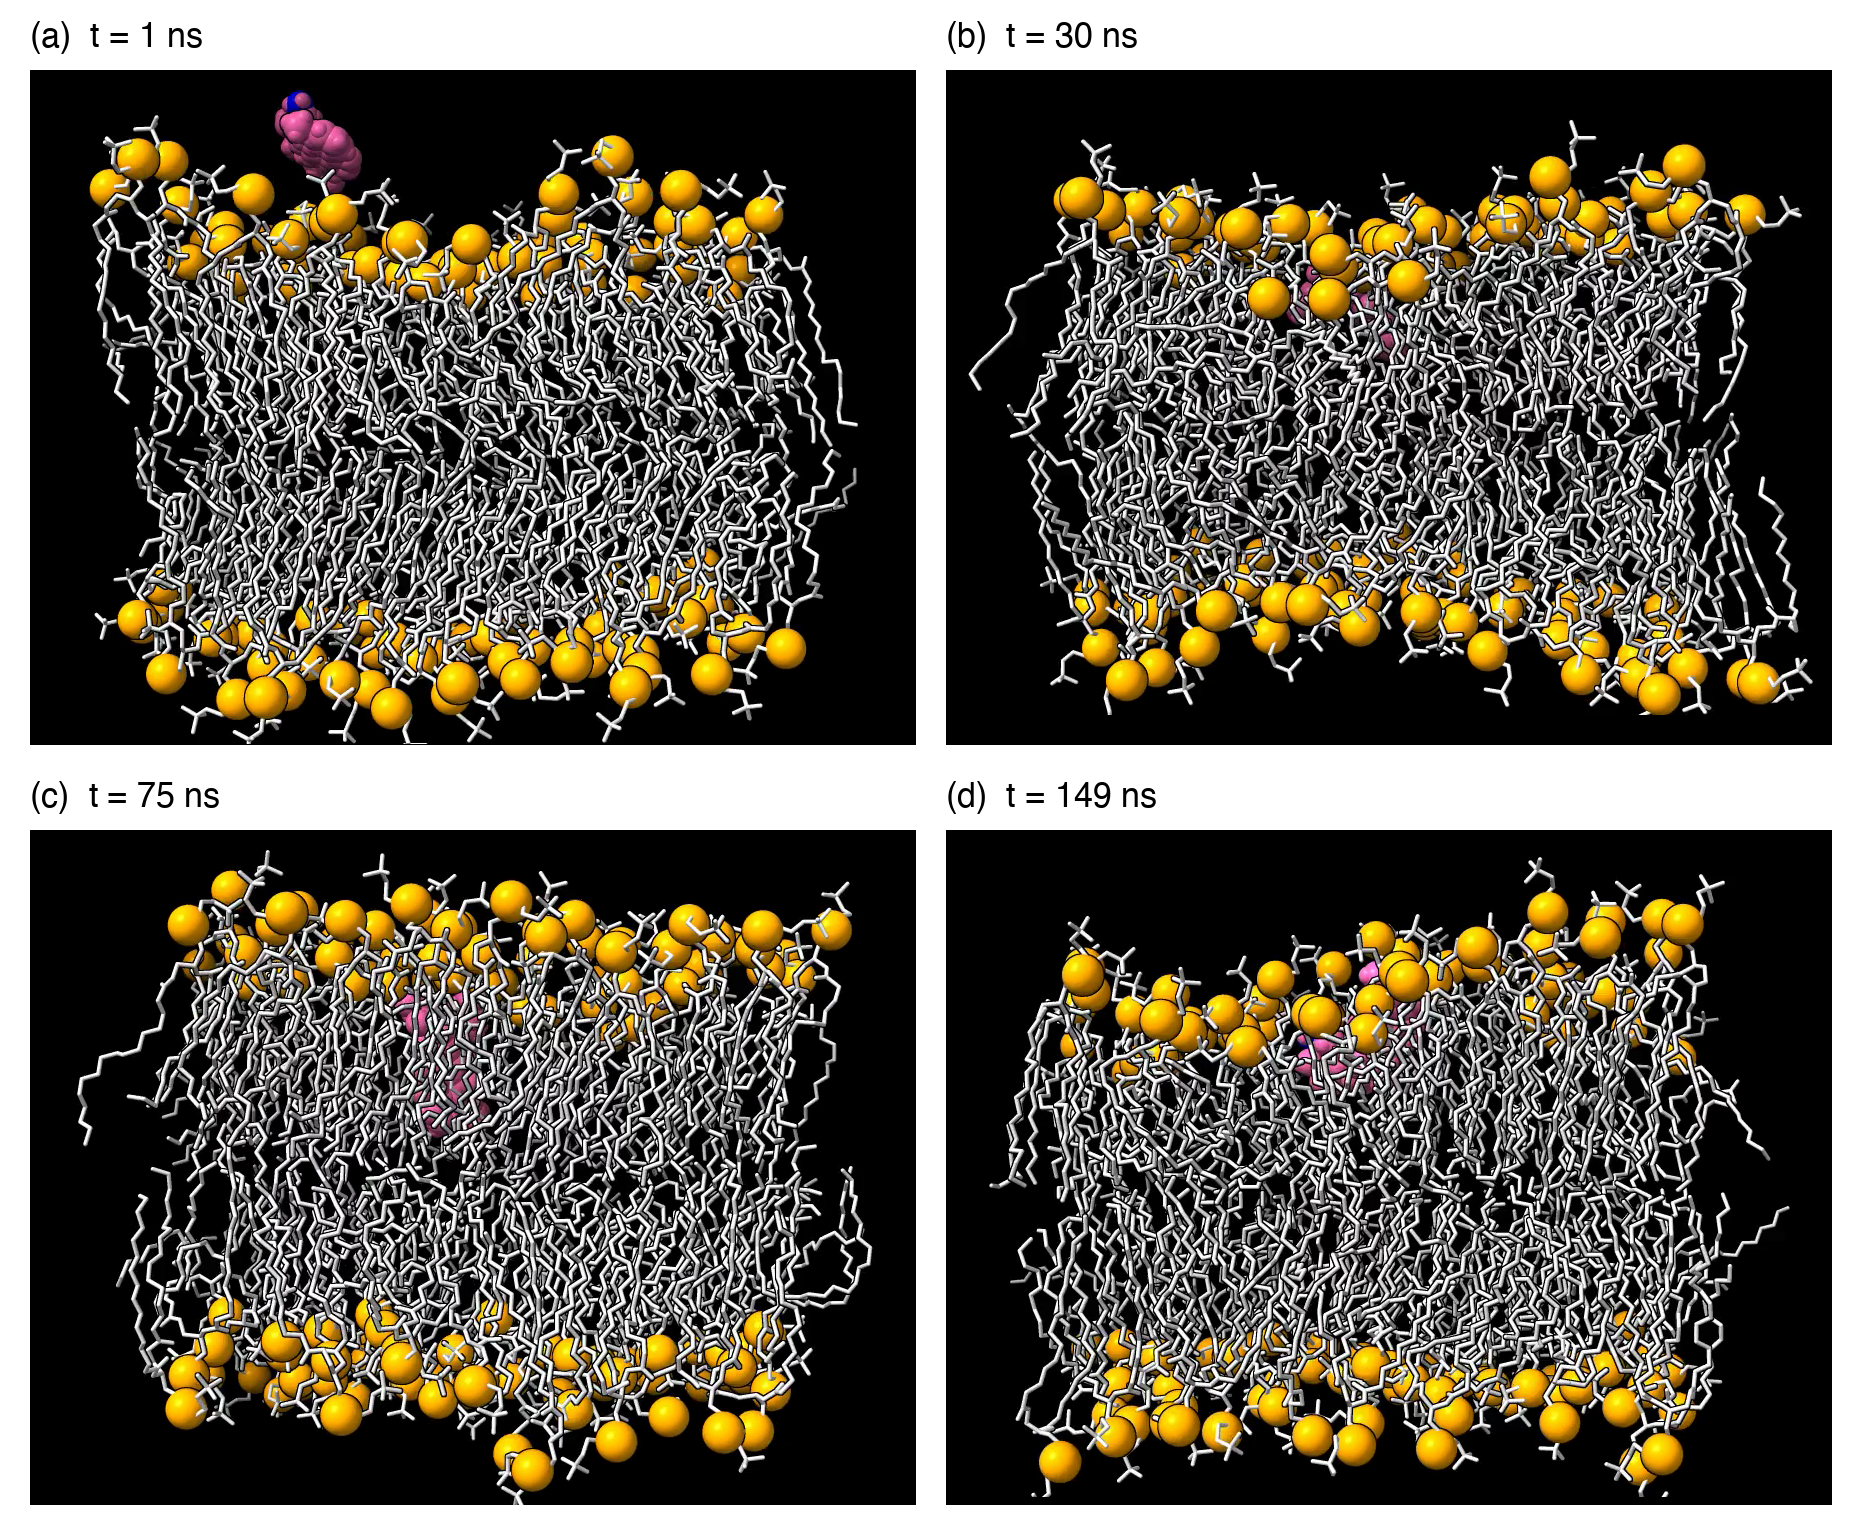
\includegraphics[width=0.86\linewidth]{fig_snap_A.png}
\caption[Snapshots of system A]{Snapshots of system \sysA{} (fluid DPPC). DPPC is shown as grey sticks,
phosphorus atoms as orange spheres and \dox{} as pink spheres (blue: \nhthree{} nitrogen); water is
omitted. (a) The drug starts in the aqueous phase. (b) It approaches the headgroups. (c, d) After insertion
it resides below the phosphate plane, partly hidden among the acyl chains.}
\label{fig:snapA}
\end{figure}

\begin{figure}[!htbp]
\centering
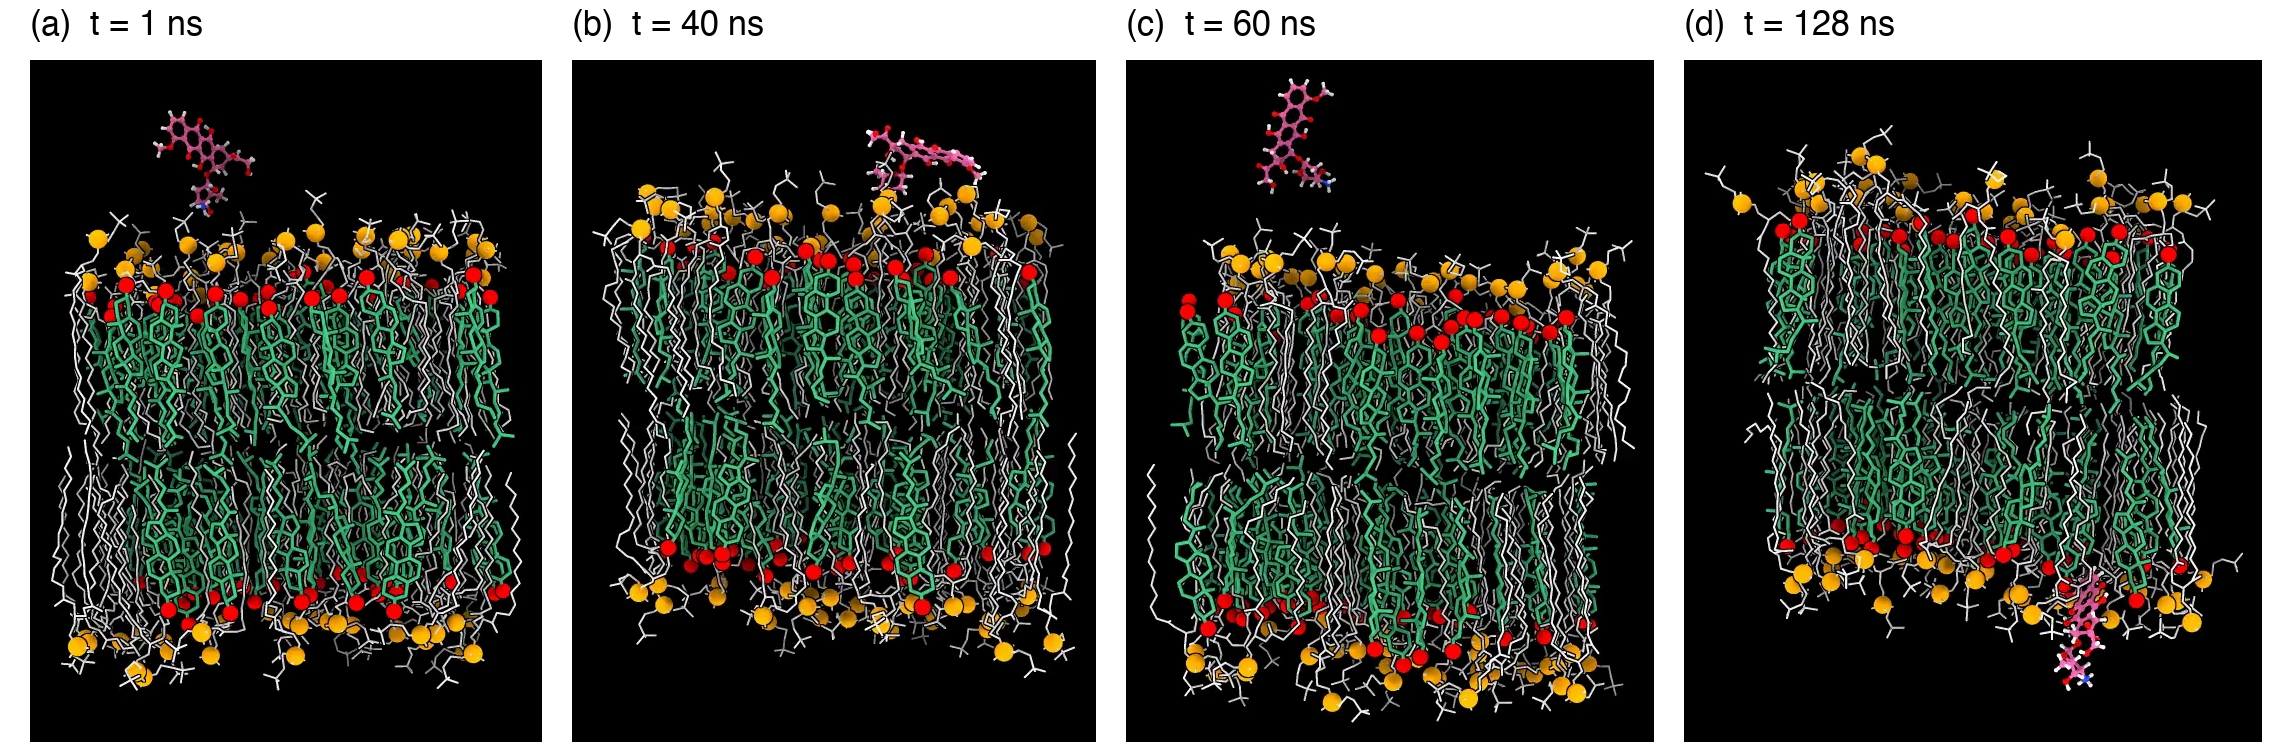
\includegraphics[width=\linewidth]{fig_snap_B.png}
\caption[Snapshots of system B]{Snapshots of system \sysB{} (DPPC/cholesterol 1:1). DPPC is shown as
white sticks, cholesterol as green sticks, cholesterol hydroxyl oxygens as red spheres, phosphorus atoms
as orange spheres and \dox{} as pink sticks. (a) Start in water. (b) Adsorbed flat on the upper headgroup
surface. (c) Desorbed back into the water. (d) Re-adsorbed on the lower leaflet. The drug never passes
the densely packed phosphate/cholesterol-hydroxyl layer.}
\label{fig:snapB}
\end{figure}

\subsection{Location within the bilayer}
Density profiles over the final bound period of each system (\cref{fig:density}) confirm the different
locations. In fluid DPPC, the \dox{} density peaks at \SI{12.5}{\angstrom} from the midplane. This is
\SI{7}{\angstrom} below the phosphate peak (\SI{19.5}{\angstrom}), in the region where the glycerol/ester
groups meet the upper acyl chains, and it overlaps strongly with the lipid-tail density. Water density
there is already low. In DPPC/cholesterol, the \dox{} peak is at \SI{29.5}{\angstrom}, which is
\SI{6}{\angstrom} \emph{outside} the phosphate peak (\SI{23.5}{\angstrom}). The drug overlaps almost
entirely with the water profile and has no overlap with the tails. The cholesterol hydroxyls form a
dense layer at \SI{18.5}{\angstrom}, just beneath the phosphates, which adds to the barrier.

\begin{figure}[!htbp]
\centering
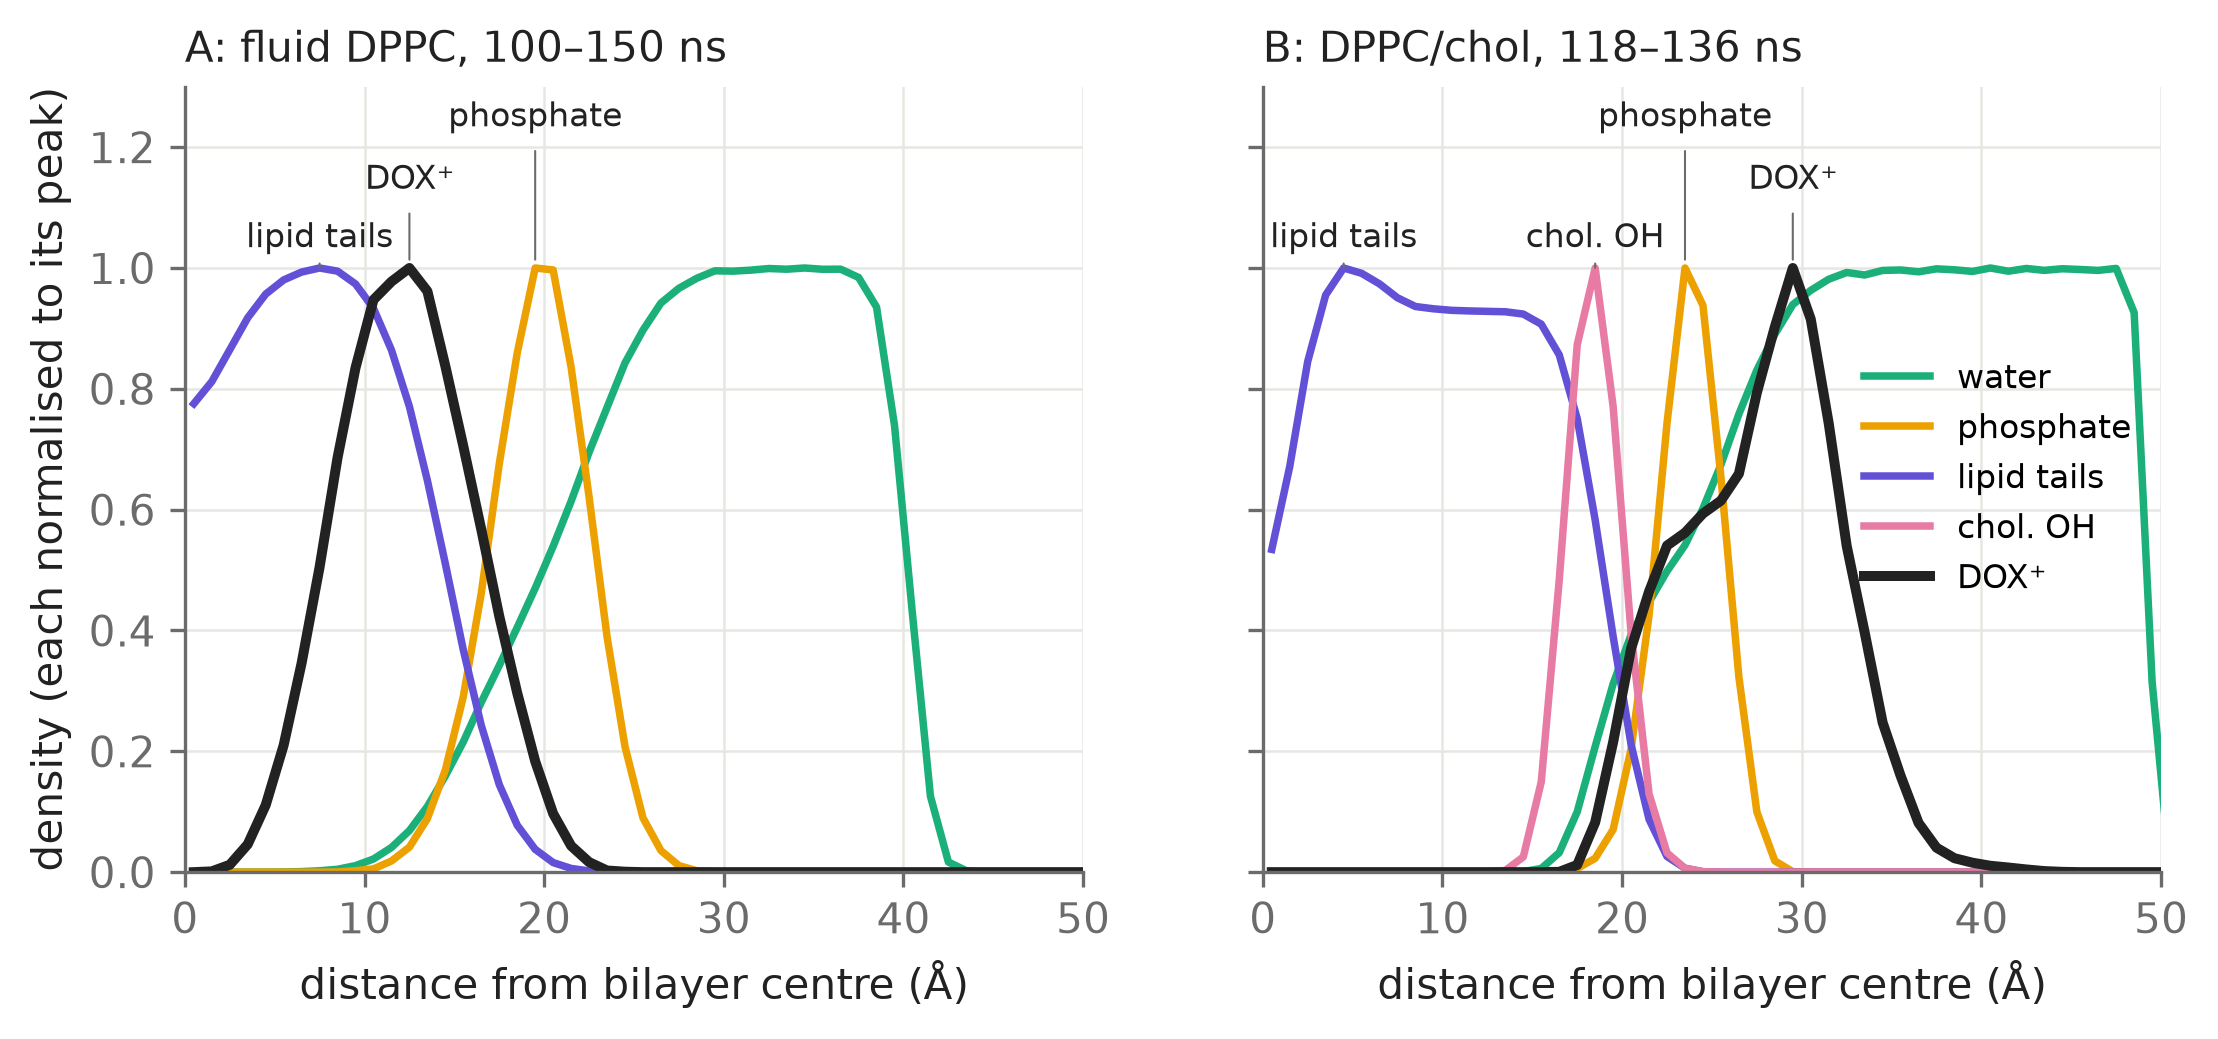
\includegraphics[width=0.98\linewidth]{fig3_density_profiles.png}
\caption[Density profiles]{Symmetrised number-density profiles along the bilayer normal, each normalised to
its own peak. Left: fluid DPPC, \SIrange{100}{150}{ns}; \dox{} lies within the membrane, between the
phosphates and the tail region. Right: DPPC/cholesterol, \SIrange{118}{136}{ns} (longest bound period);
\dox{} remains on the water side of the phosphate layer.}
\label{fig:density}
\end{figure}

\subsection{Orientation of the inserted drug}
The orientation analysis (\cref{tab:orient}) shows how \dox{} sits in each membrane. In fluid DPPC,
the \nhthree{} nitrogen remains at the phosphate/glycerol level (\SIrange{15}{18.5}{\angstrom}). The
far end of the anthracycline ring dips deeper, to \SIrange{9}{12.5}{\angstrom}, inside the upper acyl
chains. The molecule is tilted by \SIrange{40}{77}{\degree} from the bilayer normal and becomes more
parallel to the membrane plane as insertion proceeds.

This is an ``anchor-and-dip'' geometry. The charged sugar stays hydrogen-bonded to the polar interface,
while the hydrophobic aglycone is buried among the chains, consistent with the two-site model
proposed experimentally \cite{siani2021}. In DPPC/cholesterol, the whole molecule stays above the
phosphates: the ring end sits at \SI{24.6}{\angstrom}, right at the phosphate plane, and lies at
\SI{68}{\degree} to the normal, i.e.\ nearly flat on the surface.

\begin{table}[!htbp]
\centering
\caption[Orientation of \dox]{Heights above the bilayer midplane of the \nhthree{} nitrogen, the \dox{}
centre and the ring end (heavy atom farthest from N), and the angle of the N$\to$ring vector to the inward
normal ($\SI{0}{\degree}$: ring pointing straight into the membrane; $\SI{90}{\degree}$: parallel to the
surface). Phosphate plane: \SI{19.8}{\angstrom} (\sysA), \SI{23.7}{\angstrom} (\sysB).}
\label{tab:orient}
\begin{tabular}{@{}llcccc@{}}
\toprule
System & Window (ns) & N (\si{\angstrom}) & Centre (\si{\angstrom}) & Ring end (\si{\angstrom}) & Angle \\
\midrule
\multirow{3}{*}{\sysA{} DPPC} & 60--90   & 18.5 & 15.4 & 9.1  & \SI{40}{\degree} \\
                              & 90--120  & 15.3 & 12.6 & 12.5 & \SI{77}{\degree} \\
                              & 120--150 & 17.0 & 12.8 & 10.2 & \SI{57}{\degree} \\
\midrule
\sysB{} DPPC/chol             & 118--136 & 29.3 & 27.5 & 24.6 & \SI{68}{\degree} \\
\bottomrule
\end{tabular}
\end{table}

\subsection{Interaction energetics}
\Cref{fig:energy} and \cref{tab:energy} show the short-range interaction energy between \dox{} and
the membrane. In fluid DPPC, the electrostatic term becomes strongly negative as soon as the drug binds
permanently ($\approx\SI{40}{ns}$ onwards). The van der Waals term then falls sharply, from about
\SI{-5}{\kcal\per\mol} to \SI{-40}{\kcal\per\mol}, at \SI{56}{\ns}, precisely when the drug crosses the
phosphate plane.

The insertion step is therefore driven by hydrophobic (dispersion) contact between the aglycone and the
acyl chains, while the earlier anchoring is electrostatic. In the inserted state, the two contributions
are comparable: \SI{-47 \pm 18}{\kcal\per\mol} (Coulomb) and \SI{-44 \pm 7}{\kcal\per\mol} (LJ). The
LJ value agrees well with the $\approx\SI{-39}{\kcal\per\mol}$ reported by Siani \emph{et~al.} for
\dox{} in fluid DPPC \cite{siani2021}.

In DPPC/cholesterol, both terms remain small and fluctuate between zero (drug in water) and
\SIrange{-20}{-70}{\kcal\per\mol} (transient Coulomb contacts). Even in the longest bound period the
total is only about \SI{-38}{\kcal\per\mol}, against $\approx\SI{-91}{\kcal\per\mol}$ in fluid DPPC.
Almost all of it comes from DPPC; cholesterol contributes only \SI{-4}{\kcal\per\mol}, because its
hydroxyl groups lie beneath the phosphates, out of the drug's reach.

\begin{figure}[!htbp]
\centering
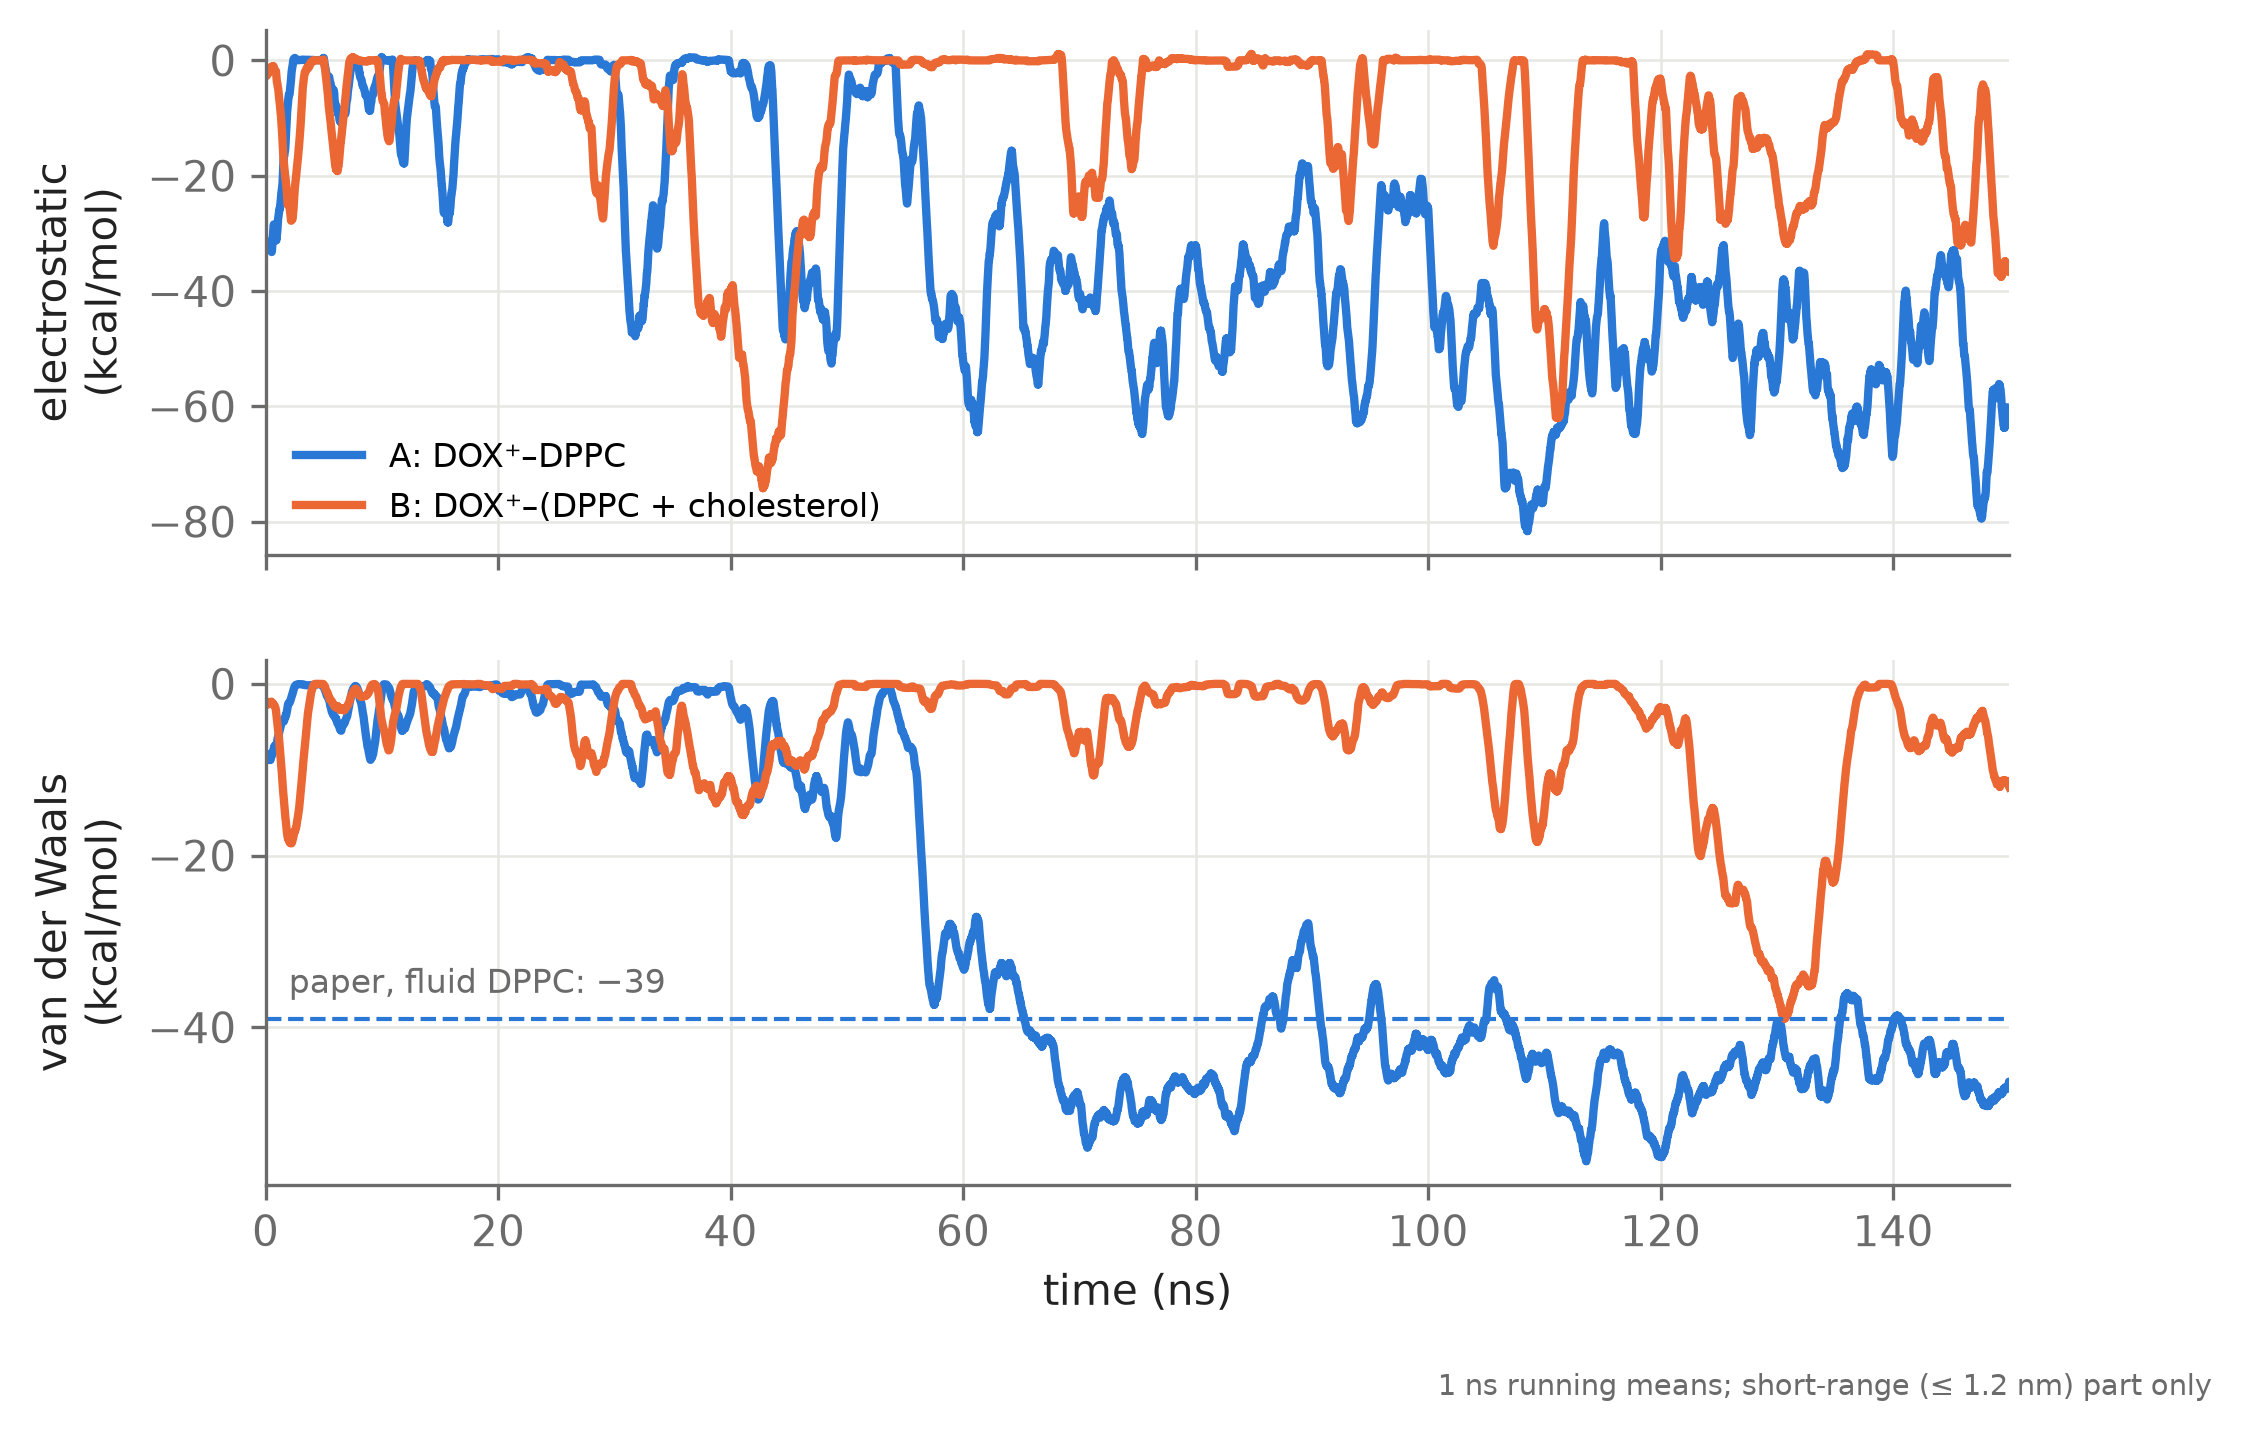
\includegraphics[width=0.92\linewidth]{fig6_interaction_energy.png}
\caption[\dox--membrane interaction energies]{Short-range electrostatic (top) and van der Waals (bottom)
interaction energy between \dox{} and the membrane (1-ns running means). In fluid DPPC (blue) the van der
Waals energy drops abruptly at insertion ($\approx\SI{56}{ns}$) to a level close to the reference value
(dashed). In DPPC/cholesterol (orange) both terms remain weak and intermittent.}
\label{fig:energy}
\end{figure}

\begin{table}[!htbp]
\centering
\caption[Interaction energies]{Average short-range \dox{}--membrane interaction energies
(\si{\kcal\per\mol}, mean $\pm$ s.d.). The PME reciprocal-space part cannot be decomposed by group and is
not included.}
\label{tab:energy}
\begin{tabular}{@{}llccc@{}}
\toprule
System & Window & Coulomb & Lennard-Jones & Total \\
\midrule
\multirow{3}{*}{\sysA{} DPPC} & 0--50 ns (before insertion) & \num{-10.6 \pm 17.6} & \num{-3.9 \pm 5.1} & $-14.5$ \\
                              & 60--150 ns (inserted)       & \num{-47.0 \pm 18.3} & \num{-44.0 \pm 6.9} & $-91.0$ \\
                              & 100--150 ns                 & \num{-52.7 \pm 17.6} & \num{-44.9 \pm 6.0} & $-97.6$ \\
\midrule
\multirow{4}{*}{\sysB{} DPPC/chol} & 0--50 ns               & \num{-14.4 \pm 21.6} & \num{-5.0 \pm 5.6}  & $-19.4$ \\
                                   & 60--150 ns             & \num{-9.8 \pm 15.1}  & \num{-6.7 \pm 9.9}  & $-16.5$ \\
                                   & 118--136 ns (bound)    & \num{-16.8 \pm 12.7} & \num{-20.9 \pm 12.3} & $-37.7$ \\
                                   & \quad of which cholesterol & $-0.8$ & $-3.3$ & $-4.1$ \\
\midrule
Siani \emph{et al.}, DPPC \Ld & last \SI{100}{ns} & -- & $\approx -39$ & -- \\
\bottomrule
\end{tabular}
\end{table}

\subsection{Molecular interactions: RDFs and hydrogen bonds}
The RDFs between the \dox{} ammonium nitrogen and the main oxygen acceptors (\cref{fig:rdf}) identify
the specific contacts. In all cases the first and dominant peak is with the phosphate oxygens, at
\SIrange{2.65}{2.75}{\angstrom}. This matches the \SI{2.65}{\angstrom} of the reference study
\cite{siani2021} and corresponds to direct \nhthree{}$\cdots$O\textsuperscript{$-$}--P salt-bridge
hydrogen bonds.

The systems differ in their second-shell partners:
\begin{itemize}
  \item In fluid DPPC, a strong peak with the \emph{ester} oxygens appears at \SI{2.75}{\angstrom}
        ($g\approx14$). Only an inserted drug can reach these carbonyl/glycerol oxygens, which lie below
        the phosphates; the reference study observed the same interaction for the \Ld{} phase.
  \item In DPPC/cholesterol, the ester and cholesterol-hydroxyl RDFs have no contact peak at all (first
        maxima beyond \SI{9}{\angstrom}). The \nhthree{}--water peak, by contrast, is higher than in
        DPPC: the drug remains fully solvated.
\end{itemize}

The hydrogen-bond counts (\cref{fig:hbonds}) tell the same story. Inserted \dox{} in DPPC donates
$\approx1.1$ hydrogen bonds per frame to phosphate oxygens and up to 0.8 to ester oxygens, with fewer
bonds to water. In the cholesterol-rich membrane, ester hydrogen bonds are essentially absent ($\le0.01$),
and water dominates (2.5--3.1 per frame). In the late bound period, even the phosphate contacts weaken to
0.3 per frame, because the drug lies flat on the surface.

\begin{figure}[!htbp]
\centering
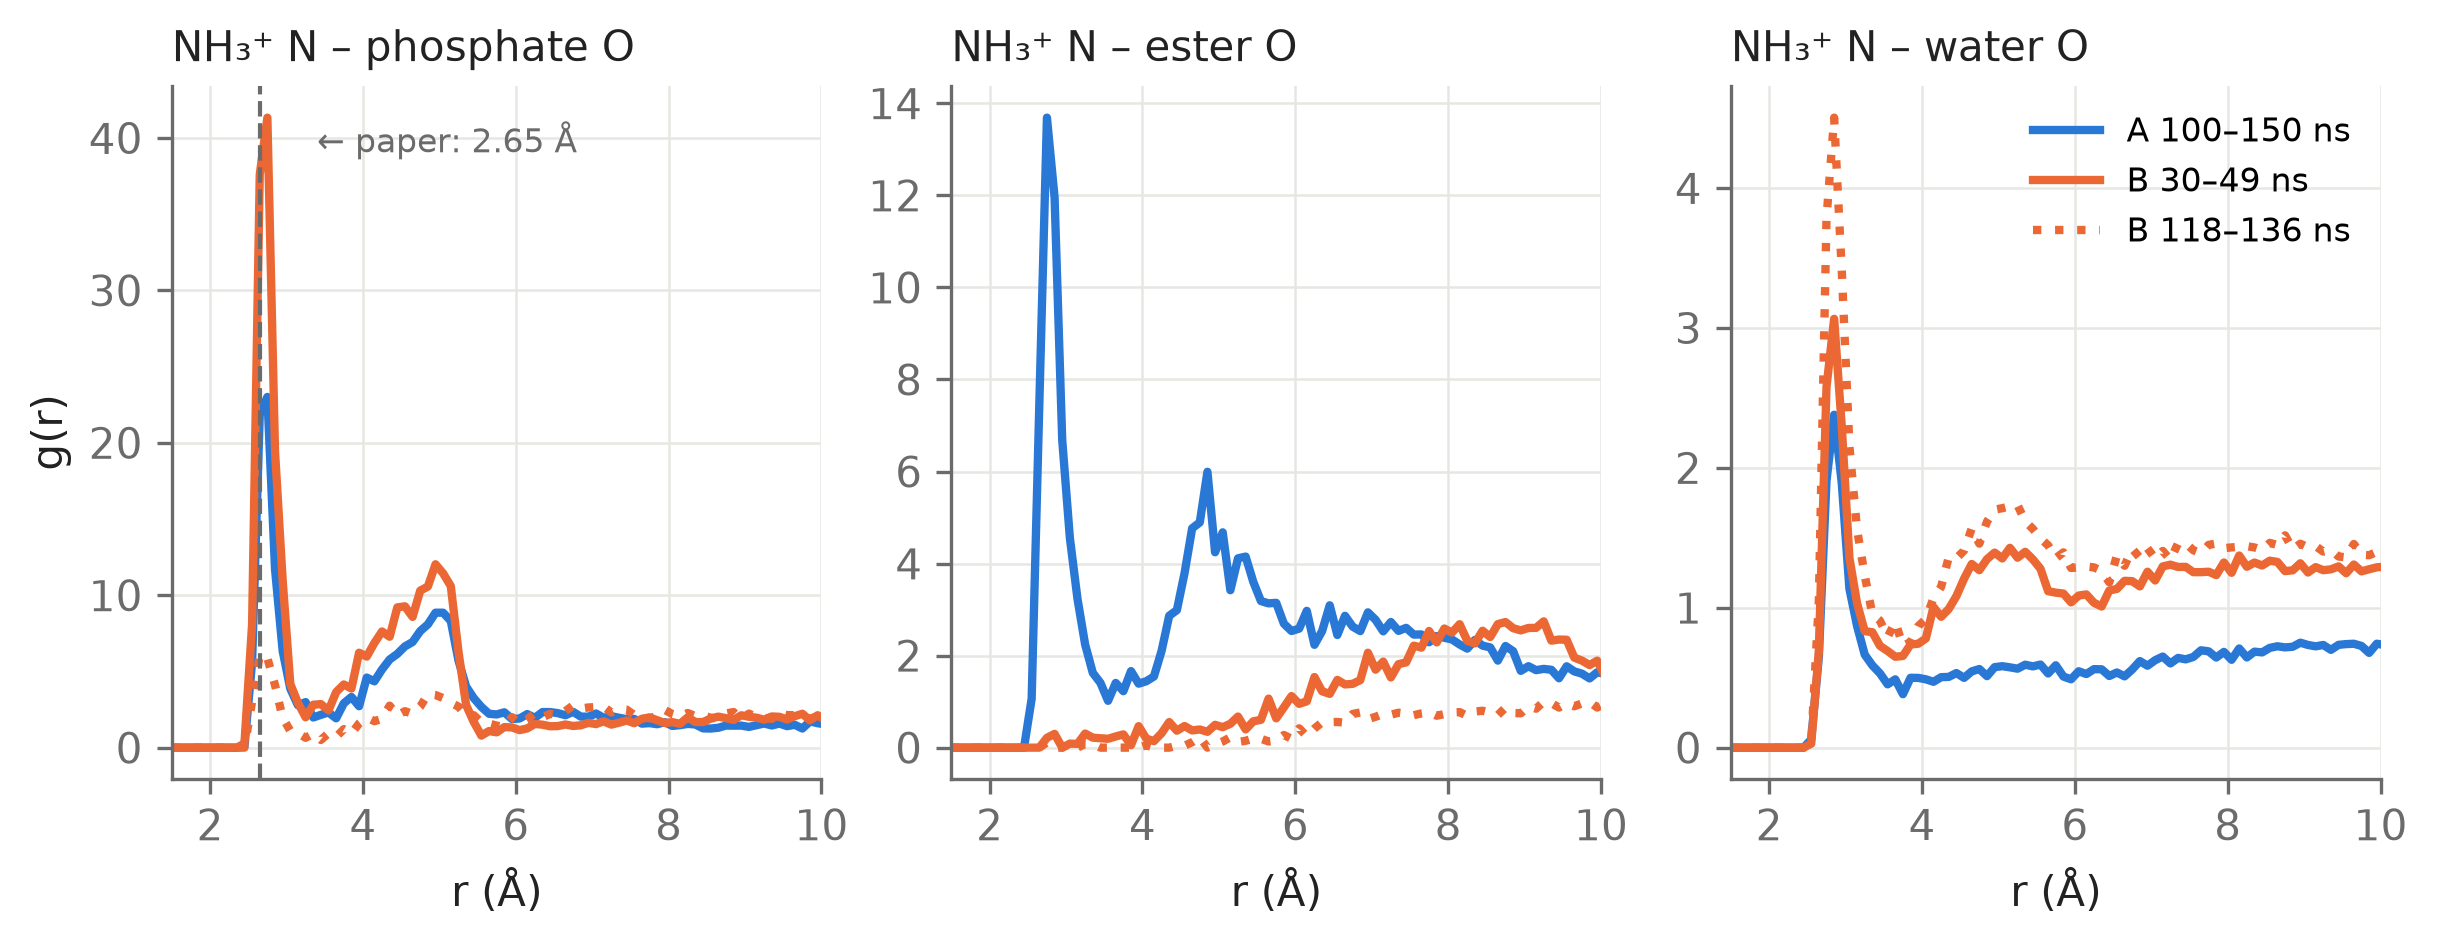
\includegraphics[width=\linewidth]{fig4_rdf.png}
\caption[Radial distribution functions]{RDFs between the \dox{} \nhthree{} nitrogen and phosphate
oxygens (left), ester oxygens (centre) and water oxygens (right). The dashed line marks the
\SI{2.65}{\angstrom} contact reported by Siani \emph{et~al.} The ester contact peak exists only for the
inserted drug in fluid DPPC.}
\label{fig:rdf}
\end{figure}

\begin{figure}[!htbp]
\centering
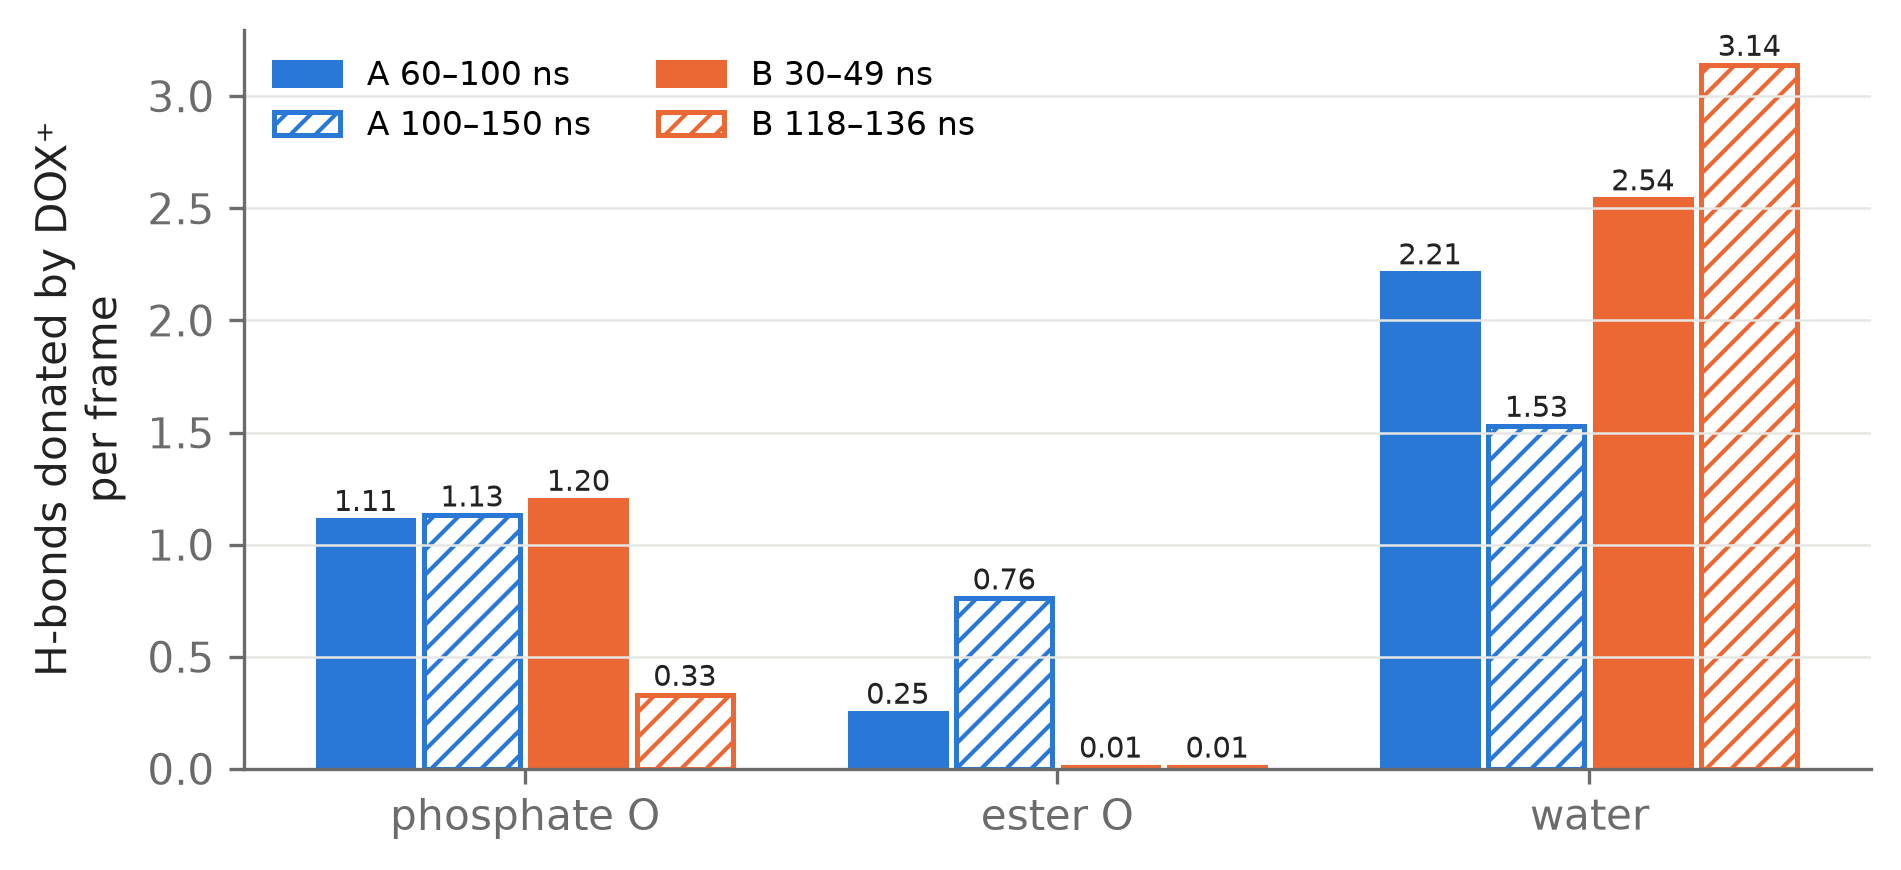
\includegraphics[width=0.82\linewidth]{fig7_hbonds.png}
\caption[Hydrogen bonds donated by \dox]{Mean number of hydrogen bonds donated by \dox{} (ammonium and
hydroxyl groups) per frame to phosphate oxygens, ester oxygens and water, in two windows per system.
Penetration into fluid DPPC replaces water hydrogen bonds by lipid-ester hydrogen bonds; in
DPPC/cholesterol the drug remains water-bonded.}
\label{fig:hbonds}
\end{figure}

\subsection{Mobility of the drug}
The lateral diffusion coefficients (\cref{fig:diffusion}) quantify how the environment of \dox{} changes.
In bulk water, $D \approx (35\text{--}96)\times10^{-7}\,\mathrm{cm^2\,s^{-1}}$, the expected magnitude for
a solute of this size in TIP3P water (which diffuses somewhat faster than real water). When the drug is
adsorbed on the cholesterol-rich surface, $D$ drops to $(5\text{--}6)\times10^{-7}\,\mathrm{cm^2\,s^{-1}}$.
After insertion into fluid DPPC, $D$ falls further, to $(0.8\text{--}2.1)\times10^{-7}\,\mathrm{cm^2\,s^{-1}}$, and decreases with time as the drug settles deeper. This is comparable
to the lateral diffusion of the lipids themselves, so the inserted drug effectively moves with the
membrane. These values derive from single trajectory segments and carry uncertainties of roughly
$\pm40\,\%$, but the differences between states span two orders of magnitude.

\begin{figure}[!htbp]
\centering
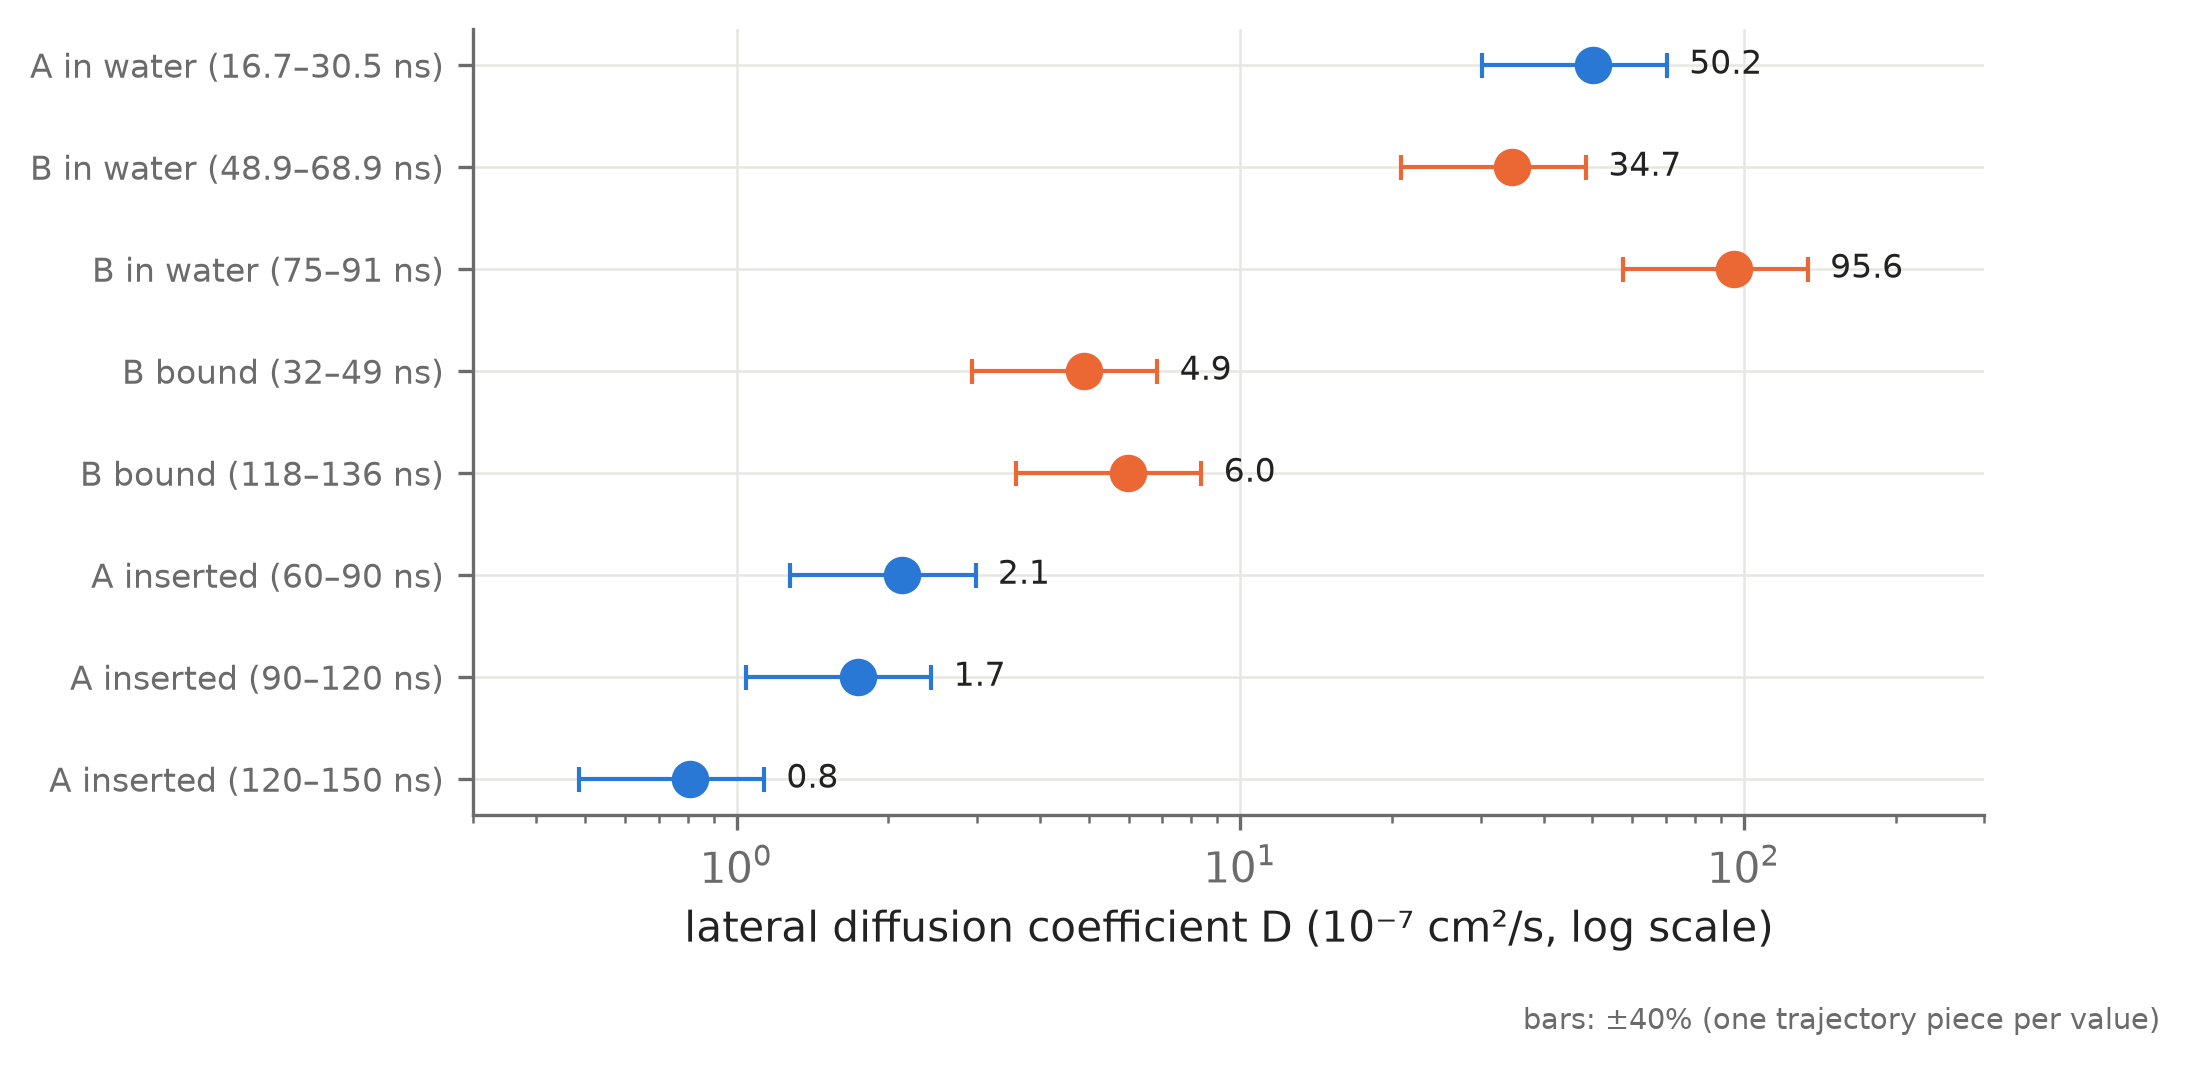
\includegraphics[width=0.85\linewidth]{fig8_diffusion.png}
\caption[Lateral diffusion of \dox]{Lateral diffusion coefficient of \dox{} in different states (log
scale). Free drug diffuses rapidly; surface adsorption on DPPC/cholesterol slows it about tenfold, and
insertion into fluid DPPC slows it about fiftyfold, to lipid-like mobility.}
\label{fig:diffusion}
\end{figure}

% =====================================================================
\section{Discussion}
\label{sec:discussion}

\subsection{Comparison with the reference study}
\Cref{tab:compare} compares the present results with those of Siani \emph{et~al.} \cite{siani2021},
who used the same force fields and membrane compositions but a different engine (NAMD),
thermostat/barostat (Langevin), and longer (\SI{500}{ns}) trajectories.

\begin{table}[!htbp]
\centering
\caption[Comparison with the reference study]{Key observables compared with Siani \emph{et~al.}
\cite{siani2021}.}
\label{tab:compare}
\begin{tabularx}{\linewidth}{@{}>{\raggedright}p{3.6cm}>{\raggedright}X>{\raggedright\arraybackslash}X@{}}
\toprule
Observable & This work (\SI{150}{ns}, GROMACS) & Siani \emph{et al.} (\SI{500}{ns}, NAMD) \\
\midrule
\nhthree{}--phosphate O contact & \SIrange{2.65}{2.75}{\angstrom} (both systems) & \SI{2.65}{\angstrom} \\
DPPC \Ld: penetration & yes, at $\approx\SI{56}{ns}$ & yes, at $\approx\SI{150}{ns}$ \\
DPPC \Ld: final location & \SI{12.5}{\angstrom} from centre; ring in upper tails & close to the tails, ring parallel to hydrocarbon region \\
DPPC \Ld: vdW energy & \SI{-44 \pm 7}{\kcal\per\mol} & $\approx\SI{-39}{\kcal\per\mol}$ \\
DPPC \Ld: \nhthree{}--ester contact & strong ($g\approx14$) & ``considerable'' \\
DPPC/chol \Lo: behaviour & reversible adsorption, no penetration & alternates water/headgroups for \SI{350}{ns}, then settles \\
DPPC/chol \Lo: final location & $\approx$\,\SI{28}{\angstrom} (above phosphates) & \SI{21.5}{\angstrom} (phosphate/ester interface) \\
\bottomrule
\end{tabularx}
\end{table}

For fluid DPPC, our results agree with the reference on every point in \cref{tab:compare}. The ammonium
group anchors to the phosphate oxygens at the same \SI{2.65}{\angstrom} distance, the drug penetrates the
bilayer, and it ends up at a similar depth with its ring tilted into the upper chains. Once inserted,
it gains a van der Waals stabilisation of similar size ($-44$ versus $\approx\SI{-39}{\kcal\per\mol}$)
and forms the same contacts with the ester oxygens. The two differences, the insertion time and the final
location in DPPC/cholesterol, are explained below.

Insertion occurred about three times earlier in our run (\SI{56}{ns} versus $\approx$\,\SI{150}{ns}). With a
single trajectory per system this is well within the stochastic spread of a rare-event waiting time.
Our drug also started closer to the membrane (\SI{29.6}{\angstrom} from the centre, versus at least
\SI{35}{\angstrom} in the reference), which shortens the initial diffusive search.

For DPPC/cholesterol, Siani \emph{et~al.} report that \dox{} ``often alternates its position between the
bulk-water phase and the headgroups in the first \SI{350}{ns}'' before settling at
\SI{21.5}{\angstrom}. Our entire \SI{150}{ns} trajectory falls within this alternating regime, and the
repeated binding and unbinding we observe (\cref{fig:timeline}) is exactly that behaviour. The
discrepancy in the final location is therefore one of sampling time rather than of physics, and it
indicates that settling at the interface in the \Lo{} phase is slower than in the \Ld{} phase.

\subsection{Analyses beyond the reference study}
\label{sec:beyond}
Siani \emph{et~al.} characterised the drug through density profiles, RDFs, hydrogen bonds and interaction
energies. This work adds several analyses that the reference study does not report:
\begin{itemize}
  \item \textbf{Acyl-chain order parameters ($\scd$; \cref{fig:scd}).} The order-parameter profiles show
        directly \emph{why} the two membranes behave so differently. Cholesterol roughly doubles the chain
        order ($-\scd$ plateau 0.43 versus 0.22), and the effect is largest at carbons 4--11, the segment
        that lies alongside the rigid cholesterol rings and just below the glycerol region. This is
        exactly the depth at which the drug's ring sits once it has inserted into fluid DPPC
        (\SIrange{9}{12.5}{\angstrom} from the midplane, \cref{tab:orient}). In the cholesterol-rich
        membrane, the chains in this region are tightly packed and leave no room for the planar ring
        to slip in. The $\scd$ profile thus links the membrane's structure to the drug's failure to
        penetrate, and the same profile, together with the area per lipid and thickness
        (\cref{tab:membrane}), validates both membrane models against NMR and scattering experiments.
  \item \textbf{Binding kinetics (\cref{fig:timeline,tab:kinetics}).} Counting individual binding events,
        residence times and rebinding times turns the qualitative picture of ``alternating between water
        and headgroups'' into numbers: 12 events with a mean residence of \SI{5.1}{ns} in DPPC/cholesterol.
  \item \textbf{Orientation angle (\cref{tab:orient}).} The tilt of the drug relative to the membrane
        normal quantifies the anchor-and-dip geometry in fluid DPPC and the flat, surface-adsorbed
        geometry in DPPC/cholesterol.
  \item \textbf{Lateral diffusion (\cref{fig:diffusion}).} The diffusion coefficient falls about tenfold
        when the drug adsorbs on the surface and about fiftyfold when it inserts, which gives an
        independent dynamical signature of each binding state.
\end{itemize}

\subsection{Mechanism and the role of cholesterol}
The results suggest a consistent mechanism for \dox{} uptake by a phosphatidylcholine membrane:
\begin{enumerate}[label=\arabic*.]
  \item \textbf{Electrostatic capture.} Long-range attraction between the cationic \nhthree{} and the
        phosphate dipoles brings the drug to the surface, where it forms a salt bridge at
        \SI{2.7}{\angstrom}.
  \item \textbf{Anchoring.} With the sugar bound, the drug samples the interface, and transient binding
        lasts a few nanoseconds.
  \item \textbf{Hydrophobic insertion.} If lipid packing leaves enough free area, the aglycone slips
        past the headgroups into the glycerol/upper-chain region. The van der Waals interaction then
        increases tenfold, and the ammonium group gains additional hydrogen bonds to the ester
        oxygens. The drug becomes trapped and adopts lipid-like mobility.
\end{enumerate}

Cholesterol blocks step 3. In the \Lo{} phase the area per molecule is 36\,\% smaller, the chains are
twice as ordered, and the space beneath the phosphates is occupied by the rigid cholesterol rings and a
dense layer of cholesterol hydroxyls. The packing defects through which the planar aglycone enters fluid
DPPC are therefore largely absent. The drug can only adsorb onto the headgroups, an interaction weak
enough (apparent $\Delta G \approx 0$) that it desorbs every few nanoseconds.

The same physical picture is consistent with:
\begin{itemize}
  \item experiments showing enhanced DOX penetration into fluid-phase PC liposomes and reduced
        interaction upon cholesterol addition \cite{siani2021,alves2017};
  \item free-energy calculations showing a higher translocation barrier at higher cholesterol content
        \cite{yacoub2011};
  \item the reference conclusion that \dox{} penetration is favoured in less tightly packed membranes
        \cite{siani2021}.
\end{itemize}

\subsection{Implications for liposomal formulation}
For a drug carrier, membrane penetration is a double-edged property. A drug that inserts readily into the
bilayer, as \dox{} does into fluid DPPC, will partition into and through the membrane and so tend to leak
from the aqueous core. A cholesterol-rich \Lo{} membrane keeps \dox{} at the surface and on the water
side. This is consistent with the high cholesterol content of clinical formulations such as Doxil, which
are designed for stable retention during circulation \cite{barenholz2012}.

Conversely, release at the target requires the barrier to be lowered, for example by a phase transition
or by pH-triggered changes in packing. Our results indicate that lipid packing, rather than headgroup
chemistry alone, is the main design variable controlling drug--membrane partitioning.

\subsection{Limitations}
\begin{itemize}
  \item \textbf{Sampling.} Each system was simulated once, for \SI{150}{ns}. Insertion is a rare event,
        so the insertion time and the late-time location in DPPC/cholesterol carry large statistical
        uncertainty. Several independent replicas, or longer runs of at least \SI{500}{ns}, would be
        needed for quantitative kinetics.
  \item \textbf{No free energies.} The apparent binding free energies depend on box size and are only
        indicative. A proper partitioning profile would require umbrella sampling or metadynamics along
        the membrane normal.
  \item \textbf{Starting position.} The drug began closer to the membrane in system \sysA{}
        (\SI{29.6}{\angstrom}) than in \sysB{} (\SI{40.3}{\angstrom}), and it was already in brief
        contact with a headgroup at $t=0$ in \sysA{}. This shortens the approach phase but cannot cause
        the qualitative difference, because \dox{} reached the \sysB{} surface 12 times without
        inserting.
  \item \textbf{Two variables changed at once.} Systems \sysA{} and \sysB{} differ in both
        cholesterol content and temperature (\SI{323}{K} versus \SI{303}{K}), as in the reference design.
        The effect of cholesterol on fluid DPPC at the same temperature was not isolated.
  \item \textbf{Force field.} \dox{} parameters come from CGenFF by analogy (penalties 28.5 and 8.7)
        without further optimisation, whereas the reference study refitted the partial charges. The
        drug was kept permanently protonated, and the single-ion system is at very low ionic strength.
  \item \textbf{Energy decomposition.} Only the short-range ($\le$\,\SI{1.2}{nm}) parts of the interaction
        energies are reported.
\end{itemize}

% =====================================================================
\section{Conclusions}
\label{sec:conclusions}
Two all-atom MD simulations of protonated doxorubicin with a fluid DPPC bilayer and an equimolar
DPPC/cholesterol bilayer were set up, validated and analysed. The main conclusions are:
\begin{enumerate}[label=\arabic*.]
  \item Both membrane models are physically sound. Fluid DPPC reproduces the experimental area per
        lipid (\SI{61.0}{} versus \SI{63.0}{\angstrom^2}), thickness and chain order. Cholesterol
        produces the expected condensing (\SI{-36}{\percent} area), thickening (\SI{+8}{\angstrom}) and
        ordering ($2\times$ $-\scd$) effects of the liquid-ordered phase.
  \item In fluid DPPC, \dox{} is captured electrostatically and then inserts spontaneously
        ($\approx$\,\SI{56}{ns}) to \SI{12}{\angstrom}--\SI{14}{\angstrom} from the bilayer centre. Its
        ammonium group stays anchored at the phosphate/ester level, and its anthracycline ring is tilted
        into the upper acyl chains. Insertion is driven by a tenfold increase in van der Waals
        stabilisation (to \SI{-44}{\kcal\per\mol}) and slows the drug's diffusion to lipid-like values.
  \item In DPPC/cholesterol, \dox{} never penetrates the membrane within \SI{150}{ns}. It adsorbs
        reversibly onto the headgroup surface, remains hydrated and interacts less than half as
        strongly with the membrane.
  \item These findings reproduce the main conclusions of Siani \emph{et~al.}: phosphate anchoring at
        \SI{2.65}{\angstrom}, penetration of the \Ld{} phase, and a vdW interaction of about
        \SI{-40}{\kcal\per\mol}. They confirm that cholesterol-induced lipid packing is the key factor
        that limits doxorubicin partitioning into phosphatidylcholine membranes.
\end{enumerate}

\section*{AI Disclosure}
\addcontentsline{toc}{section}{AI Disclosure}
AI language models (e.g.\ Claude Code) were used to improve the clarity and layout of this report and to
assist with writing the analysis and plotting scripts. All simulations were set up and run by the author,
and the author reviewed and takes full responsibility for the methods, results and conclusions presented.

% =====================================================================
\FloatBarrier
\phantomsection
\addcontentsline{toc}{section}{References}
\begin{thebibliography}{99}
\small
\bibitem{siani2021}
P.~Siani, E.~Donadoni, L.~Ferraro, F.~Re, C.~Di~Valentin,
Molecular dynamics simulations of doxorubicin in sphingomyelin-based lipid membranes,
\emph{arXiv preprint} arXiv:2109.00436v2 (2021).

\bibitem{minotti2004}
G.~Minotti, P.~Menna, E.~Salvatorelli, G.~Cairo, L.~Gianni,
Anthracyclines: molecular advances and pharmacologic developments in antitumor activity and cardiotoxicity,
\emph{Pharmacol.\ Rev.} \textbf{56} (2004) 185--229.

\bibitem{barenholz2012}
Y.~Barenholz, Doxil\textsuperscript{\textregistered}---the first FDA-approved nano-drug: lessons learned,
\emph{J.\ Control.\ Release} \textbf{160} (2012) 117--134.

\bibitem{yacoub2011}
T.~J.~Yacoub, A.~S.~Reddy, I.~Szleifer,
Structural effects and translocation of doxorubicin in a DPPC/Chol bilayer: the role of cholesterol,
\emph{Biophys.\ J.} \textbf{101} (2011) 378--385.

\bibitem{alves2017}
A.~C.~Alves, A.~Magarkar, M.~Horta, J.~L.~F.~C.~Lima, A.~Bunker, C.~Nunes, S.~Reis,
Influence of doxorubicin on model cell membrane properties: insights from \emph{in vitro} and
\emph{in silico} studies, \emph{Sci.\ Rep.} \textbf{7} (2017).

\bibitem{abraham2015}
M.~J.~Abraham, T.~Murtola, R.~Schulz, S.~P\'{a}ll, J.~C.~Smith, B.~Hess, E.~Lindahl,
GROMACS: high performance molecular simulations through multi-level parallelism from laptops to
supercomputers, \emph{SoftwareX} \textbf{1--2} (2015) 19--25.

\bibitem{jo2008}
S.~Jo, T.~Kim, V.~G.~Iyer, W.~Im,
CHARMM-GUI: a web-based graphical user interface for CHARMM,
\emph{J.\ Comput.\ Chem.} \textbf{29} (2008) 1859--1865.

\bibitem{wu2014}
E.~L.~Wu, X.~Cheng, S.~Jo, H.~Rui, K.~C.~Song, E.~M.~D\'{a}vila-Contreras, Y.~Qi, J.~Lee,
V.~Monje-Galvan, R.~M.~Venable, J.~B.~Klauda, W.~Im,
CHARMM-GUI Membrane Builder toward realistic biological membrane simulations,
\emph{J.\ Comput.\ Chem.} \textbf{35} (2014) 1997--2004.

\bibitem{lee2016}
J.~Lee, X.~Cheng, J.~M.~Swails, M.~S.~Yeom, P.~K.~Eastman, J.~A.~Lemkul, S.~Wei, J.~Buckner,
J.~C.~Jeong, Y.~Qi, S.~Jo, V.~S.~Pande, D.~A.~Case, C.~L.~Brooks~III, A.~D.~MacKerell~Jr.,
J.~B.~Klauda, W.~Im,
CHARMM-GUI Input Generator for NAMD, GROMACS, AMBER, OpenMM, and CHARMM/OpenMM simulations using the
CHARMM36 additive force field, \emph{J.\ Chem.\ Theory Comput.} \textbf{12} (2016) 405--413.

\bibitem{kim2017}
S.~Kim, J.~Lee, S.~Jo, C.~L.~Brooks~III, H.~S.~Lee, W.~Im,
CHARMM-GUI Ligand Reader and Modeler for CHARMM force field generation of small molecules,
\emph{J.\ Comput.\ Chem.} \textbf{38} (2017) 1879--1886.

\bibitem{klauda2010}
J.~B.~Klauda, R.~M.~Venable, J.~A.~Freites, J.~W.~O'Connor, D.~J.~Tobias, C.~Mondragon-Ramirez,
I.~Vorobyov, A.~D.~MacKerell~Jr., R.~W.~Pastor,
Update of the CHARMM all-atom additive force field for lipids: validation on six lipid types,
\emph{J.\ Phys.\ Chem.\ B} \textbf{114} (2010) 7830--7843.

\bibitem{vanommeslaeghe2010}
K.~Vanommeslaeghe, E.~Hatcher, C.~Acharya, S.~Kundu, S.~Zhong, J.~Shim, E.~Darian, O.~Guvench,
P.~Lopes, I.~Vorobyov, A.~D.~MacKerell~Jr.,
CHARMM general force field: a force field for drug-like molecules compatible with the CHARMM all-atom
additive biological force fields, \emph{J.\ Comput.\ Chem.} \textbf{31} (2010) 671--690.

\bibitem{jorgensen1983}
W.~L.~Jorgensen, J.~Chandrasekhar, J.~D.~Madura, R.~W.~Impey, M.~L.~Klein,
Comparison of simple potential functions for simulating liquid water,
\emph{J.\ Chem.\ Phys.} \textbf{79} (1983) 926--935.

\bibitem{steinbach1994}
P.~J.~Steinbach, B.~R.~Brooks,
New spherical-cutoff methods for long-range forces in macromolecular simulation,
\emph{J.\ Comput.\ Chem.} \textbf{15} (1994) 667--683.

\bibitem{essmann1995}
U.~Essmann, L.~Perera, M.~L.~Berkowitz, T.~Darden, H.~Lee, L.~G.~Pedersen,
A smooth particle mesh Ewald method, \emph{J.\ Chem.\ Phys.} \textbf{103} (1995) 8577--8593.

\bibitem{bussi2007}
G.~Bussi, D.~Donadio, M.~Parrinello,
Canonical sampling through velocity rescaling, \emph{J.\ Chem.\ Phys.} \textbf{126} (2007) 014101.

\bibitem{bernetti2020}
M.~Bernetti, G.~Bussi,
Pressure control using stochastic cell rescaling, \emph{J.\ Chem.\ Phys.} \textbf{153} (2020) 114107.

\bibitem{hess1997}
B.~Hess, H.~Bekker, H.~J.~C.~Berendsen, J.~G.~E.~M.~Fraaije,
LINCS: a linear constraint solver for molecular simulations,
\emph{J.\ Comput.\ Chem.} \textbf{18} (1997) 1463--1472.

\bibitem{michaudagrawal2011}
N.~Michaud-Agrawal, E.~J.~Denning, T.~B.~Woolf, O.~Beckstein,
MDAnalysis: a toolkit for the analysis of molecular dynamics simulations,
\emph{J.\ Comput.\ Chem.} \textbf{32} (2011) 2319--2327.

\bibitem{gowers2016}
R.~J.~Gowers, M.~Linke, J.~Barnoud, T.~J.~E.~Reddy, M.~N.~Melo, S.~L.~Seyler, J.~Doma\'{n}ski,
D.~L.~Dotson, S.~Buchoux, I.~M.~Kenney, O.~Beckstein,
MDAnalysis: a Python package for the rapid analysis of molecular dynamics simulations,
in \emph{Proc.\ 15th Python in Science Conf.} (2016) 98--105.

\bibitem{hunter2007}
J.~D.~Hunter, Matplotlib: a 2D graphics environment,
\emph{Comput.\ Sci.\ Eng.} \textbf{9} (2007) 90--95.

\bibitem{rdkit}
RDKit: open-source cheminformatics software, \url{https://www.rdkit.org}.

\bibitem{pubchem2023}
S.~Kim, J.~Chen, T.~Cheng, A.~Gindulyte, J.~He, S.~He, Q.~Li, B.~A.~Shoemaker, P.~A.~Thiessen,
B.~Yu, L.~Zaslavsky, J.~Zhang, E.~E.~Bolton,
PubChem 2023 update, \emph{Nucleic Acids Res.} \textbf{51} (2023) D1373--D1380.

\bibitem{pettersen2021}
E.~F.~Pettersen, T.~D.~Goddard, C.~C.~Huang, E.~C.~Meng, G.~S.~Couch, T.~I.~Croll, J.~H.~Morris,
T.~E.~Ferrin,
UCSF ChimeraX: structure visualization for researchers, educators, and developers,
\emph{Protein Sci.} \textbf{30} (2021) 70--82.

\bibitem{kucerka2011}
N.~Ku\v{c}erka, M.-P.~Nieh, J.~Katsaras,
Fluid phase lipid areas and bilayer thicknesses of commonly used phosphatidylcholines as a function of
temperature, \emph{Biochim.\ Biophys.\ Acta -- Biomembr.} \textbf{1808} (2011) 2761--2771.

\bibitem{seelig1974}
A.~Seelig, J.~Seelig,
The dynamic structure of fatty acyl chains in a phospholipid bilayer measured by deuterium magnetic
resonance, \emph{Biochemistry} \textbf{13} (1974) 4839--4845.

\bibitem{vermeer2007}
L.~S.~Vermeer, B.~L.~de~Groot, V.~R\'{e}at, A.~Milon, J.~Czaplicki,
Acyl chain order parameter profiles in phospholipid bilayers: computation from molecular dynamics
simulations and comparison with \textsuperscript{2}H NMR experiments,
\emph{Eur.\ Biophys.\ J.} \textbf{36} (2007) 919--931.
\end{thebibliography}

% =====================================================================
\clearpage
\appendix
\section{Production run parameter file}
\label{app:mdp}
The production parameter file used for system \sysA{} (\texttt{prod\_A.mdp}); system \sysB{} differs only in
\texttt{ref\_t = 303.15 303.15}.
\begin{lstlisting}
integrator              = md
dt                      = 0.002
nsteps                  = 50000000
nstxout-compressed      = 5000
nstcalcenergy           = 100
nstenergy               = 1000
nstlog                  = 1000
cutoff-scheme           = Verlet
nstlist                 = 20
rlist                   = 1.2
vdwtype                 = Cut-off
vdw-modifier            = Force-switch
rvdw_switch             = 1.0
rvdw                    = 1.2
coulombtype             = PME
rcoulomb                = 1.2
tcoupl                  = v-rescale
tc_grps                 = MEMB SOLV
tau_t                   = 1.0 1.0
ref_t                   = 323.15 323.15
pcoupl                  = C-rescale
pcoupltype              = semiisotropic
tau_p                   = 5.0
compressibility         = 4.5e-5  4.5e-5
ref_p                   = 1.0     1.0
constraints             = h-bonds
constraint_algorithm    = LINCS
continuation            = yes
nstcomm                 = 100
comm_mode               = linear
comm_grps               = MEMB SOLV
\end{lstlisting}

\section{Ligand protonation script}
\label{app:protonate}
\begin{lstlisting}[language=Python]
from rdkit import Chem
from rdkit.Chem import AllChem
import sys

infile, outfile = sys.argv[1], sys.argv[2]
mol = Chem.SDMolSupplier(infile, removeHs=False)[0]
print("input atoms:", mol.GetNumAtoms(), Chem.rdMolDescriptors.CalcMolFormula(mol))

# strip H, protonate the primary amine, put all H back with 3D coordinates
mol = Chem.RemoveHs(mol)
matches = mol.GetSubstructMatches(Chem.MolFromSmarts("[NX3;H2;!$(N-C=O)]"))
assert len(matches) == 1, f"expected exactly 1 primary amine, found {len(matches)}"
n = mol.GetAtomWithIdx(matches[0][0])
n.SetFormalCharge(1)
n.SetNumExplicitHs(0)
n.SetNoImplicit(False)
Chem.SanitizeMol(mol)
mol = Chem.AddHs(mol, addCoords=True)

print("output atoms:", mol.GetNumAtoms(), Chem.rdMolDescriptors.CalcMolFormula(mol))
print("net charge:", Chem.GetFormalCharge(mol))
Chem.MolToMolFile(mol, outfile)
\end{lstlisting}

\section{Data and script inventory}
\label{app:files}
\begin{table}[!htbp]
\centering
\small
\begin{tabularx}{\linewidth}{@{}>{\raggedright\ttfamily}p{5.4cm}X@{}}
\toprule
\normalfont\textbf{File / folder} & \textbf{Content} \\
\midrule
DOX\_plus.sdf, protonate.py & \dox{} structure and the script that produced it \\
charmm-gui-9262145299/ & CHARMM-GUI Ligand Reader output (CGenFF topology of \dox) \\
charmm-gui-9239757263/, -9296217723/ & CHARMM-GUI Membrane Builder inputs and outputs \\
system\_A/, system\_B/ & GROMACS topologies, \texttt{.mdp} files, equilibration and production runs \\
prod\_A\_full.xtc, prod\_B\_full.xtc & concatenated \SI{150}{ns} production trajectories (\SI{10}{ps}/frame) \\
dox\_track*.csv & per-frame drug height, thickness and minimum distances \\
dens\_*.csv, rdf\_*.csv, scd\_*.csv & density profiles, RDFs, order parameters \\
energy\_A.xvg, energy\_B.xvg & \dox--membrane interaction energies from \texttt{mdrun -rerun} \\
track.py, kinetics.py, cross.py, density.py, rdf.py, hbonds.py, orient.py, msd.py, scd.py, membrane.py & analysis scripts (Python / MDAnalysis) \\
report/make\_figures.py & regenerates all data plots (Figs.~\ref{fig:scd}--\ref{fig:timeline} and \ref{fig:density}--\ref{fig:diffusion}) from the data files \\
A\_video\_150ns.mp4, B\_video\_150ns.mp4 & ChimeraX movies of the trajectories (source of the snapshots) \\
\bottomrule
\end{tabularx}
\end{table}

\end{document}
